\documentclass[11pt,a4paper]{article}
\usepackage[margin=2.2cm]{geometry}
\usepackage[T1]{fontenc}
\usepackage[utf8]{inputenc}
\usepackage{lmodern}
\usepackage{amsmath,amssymb}
\usepackage{booktabs}
\usepackage{longtable}
\usepackage{array}
\usepackage{tabularx}
\usepackage{graphicx}
\usepackage{xcolor}
\usepackage{enumitem}
\usepackage{hyperref}
\usepackage{tikz}
\usetikzlibrary{positioning,arrows.meta,fit,backgrounds,calc}
\usepackage{caption}
\usepackage{float}
\usepackage{microtype}
\usepackage{url}
\hypersetup{colorlinks=true,linkcolor=blue!60!black,citecolor=blue!60!black,urlcolor=blue!60!black,breaklinks=true}
\setlist{nosep,leftmargin=*}
\newcolumntype{L}[1]{>{\raggedright\arraybackslash}p{#1}}
\newcommand{\ok}{\textcolor{green!50!black}{\checkmark}}
\newcommand{\bad}{\textcolor{red!70!black}{\texttt{X}}}
\newcommand{\todo}[1]{\textcolor{red}{[#1]}}
\newcommand{\model}{\textsc{TomaNet}}
\newcommand{\modelcls}{\textsc{TomaNet-C}}
\newcommand{\modeldet}{\textsc{TomaNet-D}}
\usepackage{amsthm}

\title{\textbf{Tomato Leaf Disease Recognition: Research Audit, State of the Field (2026), Datasets, and a Proposed Unified Classification--Detection Pipeline}\\[4pt]
\large Working research plan}
\author{Prepared for the tomato disease detection research project}
\date{30 August 2026}

\begin{document}
\maketitle
\tableofcontents
\newpage

\section{Executive Summary}

\paragraph{Is the current approach doable?} Yes, but as stated it is not novel and the two decks contradict each other numerically. Deck~A's DenseNet121 classification and Deck~B's YOLOv8-vs-Faster-R-CNN detection are both standard 2020--2022 work; PlantVillage tomato classification is saturated (99.4--99.96\% published), and ``YOLOv8 beats Faster R-CNN'' is a known result, not a finding. Eleven concrete inconsistencies are listed in \S\ref{sec:audit} (three different accuracies for the same model, learning rates written as ``1e-4 (0.00001)'', a Grad-CAM IoU that requires lesion masks the project does not have, a ``fruit disease'' branch trained on ripeness data).

\paragraph{Where the novelty actually is.} Six verified gaps in the 2024--2026 tomato literature (\S\ref{sec:novelty}): (i) no lightweight block family evaluated as \emph{both} classifier and detector; (ii) no label-efficiency curve for self-supervised learning on tomato; (iii) no modern anomaly-detection benchmark (PatchCore/PaDiM) on tomato; (iv) no leave-one-disease-out open-set benchmark; (v) no \emph{quantitative} explainability evaluation (every tomato XAI paper shows heat-maps as figures only); (vi) no public tomato field dataset from Gujarat.

\paragraph{Datasets.} \S\ref{sec:datasets} catalogues 40+ public sets. The critical fact: the ``10\,000-image'' and ``18\,000-image'' tomato sets in both decks are the \emph{same} PlantVillage data, re-split. Real cross-domain work needs Taiwan (622 raw field images), PlantDoc, Tomato-Village (Rajasthan, has detection and multi-label variants), CCMT, FieldPlant, PlantSeg (pixel masks), plus the North-Gujarat custom set. A classifier reading only 8 background pixels of PlantVillage scores 49\%; a ResNet at F1 0.987 in-domain drops to F1 0.012 on Tomato-Village.

\paragraph{Proposed model.} \model{}: one re-parameterisable block (partial convolution + large-kernel depthwise + coordinate attention) instantiated as \modelcls{} (GAP+FC head, 224\,px) and \modeldet{} (PAFPN neck of the same block + anchor-free DFL head, 640\,px), both built inside a fork of Ultralytics so that the assigner, losses, augmentation and mAP evaluation are the standard ones. Target: $\le$5\,M params, $\le$10\,GFLOPs. Baselines span everything in the original survey (AlexNet$\to$DenseNet$\to$ViT, Faster R-CNN, YOLOv4/v5/v8) \emph{plus} the current state of the art (YOLOv10/11/12/26, RT-DETR, ConvNeXt, EfficientNetV2, RepViT, FastViT, StarNet).

\paragraph{Supervised and unsupervised.} Supervised is the backbone of the work. Unsupervised is worth doing but only in three specific forms (\S\ref{sec:unsup}): self-supervised \emph{pre-training} to cut label cost (domain SSL on 3k images beats ImageNet-21k transfer in published work), healthy-only \emph{anomaly detection} for unknown-disease flagging (AUROC 0.94--0.99 on comparable crops), and \emph{semi-supervised} pseudo-labelling. Unsupervised \emph{clustering into disease classes} does not work -- published NMI is 0.27 with ImageNet features and 0.64 with the best specialised method, because clusters follow species/colour/lighting, not pathology. Fully unsupervised lab$\to$field adaptation is also a dead end for tomato: the best published number is 50.6\%, whereas ten labelled field images per disease gives $+11$ to $+29$ F1.

\paragraph{Metrics.} \S\ref{sec:metrics} defines everything with formulas: macro-F1/$\kappa$/MCC/ECE for classification, COCO mAP with AP$_\text{small}$ for detection (lesions are small objects), params/GFLOPs/latency on GPU/CPU/edge, cross-dataset gap and corruption robustness, pointing game / energy-PG / deletion--insertion / saliency-IoU for XAI, AUROC/FPR95 for anomaly, NMI/ARI for clustering, plus McNemar and paired tests over $\ge$3 seeds.

\paragraph{Cost.} $\approx$900 GPU-hours ($\approx$6 weeks on one 12\,GB GPU), reducible to $\approx$450 by cutting seeds and the ``m'' scale. Fourteen-week timeline in \S\ref{sec:experiments}.

\paragraph{Honest expectation.} \model{} will probably \emph{not} beat YOLO11/YOLOv12 in-domain, and it does not need to. The defensible claims are Pareto efficiency at $\le$3\,M parameters, smaller cross-domain degradation, measured label efficiency, unknown-disease flagging, and quantified explanations -- plus a released dataset. Frame the paper that way from the first draft.

\section{Audit of the Current Proposal}
\label{sec:audit}

Two versions of the slide deck were supplied: Deck~A (DenseNet121 vs.\ a ``Sequential'' CNN, image classification) and Deck~B (YOLOv8 vs.\ Faster R-CNN with Grad-CAM, object detection on leaf, fruit and pest images). Both are \emph{technically executable}; the problems are in experimental protocol, internal consistency, and novelty. Table~\ref{tab:audit} lists what must be fixed before any of it can be written up.

\begin{longtable}{@{}L{0.5cm}L{5.2cm}L{5.4cm}L{5.0cm}@{}}
\caption{Issues found in Deck~A and Deck~B, with the fix adopted in this plan.}\label{tab:audit}\\
\toprule
\# & Issue & Why it matters & Fix in this plan \\
\midrule
\endfirsthead
\toprule
\# & Issue & Why it matters & Fix in this plan \\
\midrule
\endhead
\bottomrule
\endfoot
\multicolumn{4}{@{}l}{\textbf{Deck A -- DenseNet121 classification}}\\
\midrule
A1 & Three different accuracies for the same DenseNet121 run: 99.6\% (conclusion), 99.6/99.2\% train/val (results), 96.2/94\% (table). & Reviewers reject papers whose numbers disagree with themselves. & One results table, generated by a script from saved predictions; every number traceable to a run ID and seed. \\
A2 & Dataset described as ``high-resolution RGB photos captured in natural environments''. The 10\,000-image, 10-class set is a Kaggle re-split of PlantVillage: 256$\times$256 lab images on uniform backgrounds. & Mis-describing the data hides the biggest weakness (lab-only images do not transfer to the field; see \S\ref{sec:sota}). & Describe each dataset by provenance, acquisition conditions and known biases (\S\ref{sec:datasets}); add field datasets. \\
A3 & Learning rates written as ``1e-4 (0.00001)'' and ``1e-3 (0.0001)''. & Arithmetic errors in hyper-parameter tables undermine trust. & Hyper-parameters stored in a versioned YAML; table generated from it. \\
A4 & The ``Sequential'' baseline (85\%) is a straw man; the claim ``outperformed state-of-the-art'' is made without comparing to any published number. & PlantVillage-tomato classification is saturated at 99--99.9\% in the literature; 96--99\% is not a contribution. & Compare against the full baseline set in \S\ref{sec:baselines}, on identical splits, with mean$\pm$std. \\
A5 & ``When the gradient vanishing issue is fixed'' -- ReLU inside DenseNet is the stock architecture. & Presented as a contribution; it is not. & Remove. Novelty is defined in \S\ref{sec:novelty}. \\
A6 & 80/20 train/test with ``validation accuracy'' reported; no separate validation split; no repeated runs. & Model selection on the test set inflates results; a single run has no error bar. & 70/15/15 stratified split with deduplication; 5 seeds (or 5-fold CV); McNemar / paired test between models. \\
A7 & Precision 0.98, recall 0.99, F1 0.99 with accuracy 99.6\% -- inconsistent (macro-F1 cannot exceed both P and R). & Metric definitions unclear (micro vs macro). & Report macro-P/R/F1, kappa, MCC, per-class confusion matrix (\S\ref{sec:metrics}). \\
\midrule
\multicolumn{4}{@{}l}{\textbf{Deck B -- YOLOv8 / Faster R-CNN + Grad-CAM}}\\
\midrule
B1 & ``Accuracy 94\%'' reported for a detector; fruit accuracy is 87\% in the table and 89\% in the text; Grad-CAM IoU 0.40 in the table, 0.39 in the text; ``NSR'' never defined. & Accuracy is not a detection metric unless defined (image-level? box-level at which IoU?); inconsistent values. & Report COCO-style mAP@0.5, mAP@0.5:0.95, AP$_s$/AP$_m$/AP$_l$, P/R/F1 at a fixed confidence; define every XAI metric with a formula (\S\ref{sec:metrics}). \\
B2 & Grad-CAM applied to YOLOv8 without stating the target layer, the target score (class logit? objectness? which box?) or how gradients pass NMS. & Grad-CAM needs a scalar target; for one-stage detectors the standard practice is EigenCAM / Grad-CAM on the neck output for a chosen box. Unspecified = irreproducible. & Specify: EigenCAM and Grad-CAM++ on the P3/P4 neck features, target = class score of the selected box before NMS; report pointing game and energy-based pointing game against lesion masks. \\
B3 & ``Avg.\ Grad-CAM IoU 0.51'' requires ground-truth lesion masks; only boxes exist. & If IoU was computed against boxes, it is a box-IoU of a thresholded heatmap, not a lesion-localisation score. & Annotate a small lesion-mask subset (200--300 images) for XAI evaluation, or use the pixel-mask datasets in \S\ref{sec:datasets}. \\
B4 & Pipeline text describes a ``classification network with self-attention, multi-head attention and transfer learning'' after YOLOv8, but no such network appears in results. & Claimed component not evaluated. & Replace with the actual custom model (\S\ref{sec:model}); every named component gets an ablation row. \\
B5 & Faster R-CNN (2015) is the only comparator. & YOLOv8 $>$ Faster R-CNN in speed and usually mAP is a known result; not a finding. & Baselines: YOLOv5/8/10/11/12, RT-DETR, plus lightweight classifiers (\S\ref{sec:baselines}). \\
B6 & Fruit dataset is ripe/unripe (ripeness), yet results are described as ``fruit disease detection''. & Task mismatch. & Either annotate fruit disorders (blossom-end rot, cracking, sunscald) or present the fruit branch as ripeness/maturity, not disease. \\
B7 & Custom North-Gujarat set (3\,153 ``mixture'' images) has no described class list, annotation protocol, camera, season, or inter-annotator agreement. & This set is the strongest novelty asset in the whole project; undocumented it cannot be published or reused. & Dataset card + annotation protocol (\S\ref{sec:custom_dataset}); release on Zenodo/Mendeley with DOI. \\
B8 & Pre-processing says ``one-hot encoded vectors for multi-class classification'' for a detector; 640$\times$640 for classification too. & Copy--paste from Deck~A; detectors use box labels; classifiers normally use 224--384 px. & Task-specific pre-processing (\S\ref{sec:pipeline}). \\
B9 & Research-gap slide lists severity, multi-disease-per-leaf, field robustness, temporal tracking, explainability -- but the proposed method only addresses explainability (qualitatively). & Gap and method are disconnected. & Each claimed gap maps to a measurable experiment (Table~\ref{tab:gap_map}). \\
B10 & Bibliography: duplicate [21][21]; numbering differs between decks; several ``research observation'' cells contradict the paper described (e.g.\ Reis~2024 listed as KNN/SVM but described as lightweight CNN + meta-learning; Nawaz~2023 ``highly effective'' in Deck~A, ``has not proven effective'' in Deck~B). & Credibility. & BibTeX with DOIs; observation column rewritten from the actual abstracts. \\
\end{longtable}

\paragraph{Verdict on feasibility.}
\begin{itemize}
  \item \textbf{Doable now:} YOLOv8/Faster R-CNN detection with Grad-CAM (already run), DenseNet121 classification (already run).
  \item \textbf{Doable with moderate effort (2--4 months on one GPU):} the custom dual-task model of \S\ref{sec:model}, the cross-domain protocol, SSL pre-training, quantitative XAI.
  \item \textbf{Not doable as stated:} ``fruit disease'' without disease-annotated fruit; ``severity'' without lesion masks or expert severity scores; ``temporal progression'' without a time-series dataset. These are dropped or scoped down explicitly in \S\ref{sec:experiments}.
  \item \textbf{Where the novelty actually is:} (i) a single block family that instantiates both a classifier and a detector, trained under one recipe and evaluated under one protocol; (ii) a lab$\rightarrow$field generalisation study across five public datasets plus the North-Gujarat field set; (iii) self-supervised pre-training on pooled unlabelled tomato images with label-efficiency curves; (iv) healthy-only anomaly detection for \emph{unknown} disease flagging; (v) quantitative, not qualitative, explainability. No single one of these is new; the combination on tomato, with a released field dataset, is publishable.
\end{itemize}

\section{State of the Field (2023--2026)}
\label{sec:sota}

\subsection{Headline facts}
\begin{enumerate}
  \item \textbf{PlantVillage-tomato classification is solved.} 2024--2026 papers report 99.4--99.96\% (Eff-Swin 99.70\%~\cite{effswin}, MobilePlantViT 99.40\% with 0.82\,M params~\cite{hoang2026}, MobileNetV3-L 99.81\%~\cite{mnv3edge}, ViT+MoE 99.96\% on the full 38-class set~\cite{salman2025}). Differences of $<0.5$\,pp are within seed noise. A new architecture cannot be justified by PlantVillage accuracy alone.
  \item \textbf{PlantVillage is background-biased.} A classifier that sees only 8 background pixels reaches 49\% on PlantVillage (chance 2.6\%)~\cite{noyan2022}. Mohanty et al.\ (2016): 99.35\% held-out $\to$ 31.4\% on external web images~\cite{mohanty2016}. Recent lab$\to$field numbers: ViT+MoE 99.96\% $\to$ 68--74\% on PlantDoc~\cite{salman2025}; ResNet-50 PlantVillage$\to$PlantDoc $-67.7$\,pp with mean confidence still 79.8\%~\cite{fpls2026gap}; ViT-B 99.17\% $\to$ 77.27\% on an Indian field subset~\cite{eja2025}; 99.72\% $\to$ 41.81\% (field)~\cite{yang2024}. Jelali (2024) reviewed 35 tomato studies that use \emph{only} real-field data and concludes PlantVillage-trained models ``perform poorly on real-world images''~\cite{jelali2024}.
  \item \textbf{Detection has moved to field data and YOLO/RT-DETR variants.} A fair, single-recipe benchmark of YOLOv8--v12 (all sizes) on the Tomato-Village detection variant (6 classes, 14\,368 images after augmentation) gives YOLOv11x mAP@0.5 0.936 / mAP@[0.5:0.95] 0.790 and YOLOv12n 0.864 / 0.604 as the best nano model~\cite{ramos2025}. This is the number to beat, at the nano/small scale.
  \item \textbf{Typical ``improved YOLO'' paper gains are small.} Attention/neck/loss tweaks report $+1$ to $+4$ mAP@0.5 on a single dataset, single seed, e.g.\ improved YOLOv8n 80.2 $\to$ 81.8 on 20\,534 Hainan field images~\cite{chen2025yolov8n}; YOLO11n $+1.3$ on 2\,212 Sanya images~\cite{meng2025}. Reviewers are increasingly sceptical of this pattern.
  \item \textbf{Unified/multi-task models exist but are heavy.} PMJDM (ConvNeXt shared backbone, species classification + disease detection) is 49\,M params / 146\,GFLOPs~\cite{pmjdm}; multi-task disease+severity distillation~\cite{liu2024mt}; LDI-NET (type/disease/severity multi-label)~\cite{ldinet}. \emph{No lightweight ($<5$\,M) block family evaluated as both a classifier and a detector on tomato was found.}
  \item \textbf{Explainability is qualitative.} Grad-CAM / Grad-CAM++ / LIME / SHAP / Eigen-CAM appear in many tomato papers~\cite{xsetomatonet,leafdet,gunasekaran2026}, always as figures. The only quantitative saliency-vs-lesion-mask study found is on a non-tomato dataset (DeepSHAP IoU $>85\%$)~\cite{shafik2025xai}. Pointing game, energy-based pointing game and deletion/insertion curves were \emph{not} found in any tomato paper. One 2026 paper explicitly lists lack of IoU-based heat-map scoring as a limitation~\cite{scirep2026xai}.
  \item \textbf{Foundation models are arriving.} PlantCaFo (CLIP+DINO+DINOv2 adapters, 16-shot 93.5\% on 38-class PlantVillage)~\cite{plantcafo}; BLIP-2+LoRA with GroundingDINO/SAM-2 zero-shot leaf masking on tomato, 97.27\%, runs on Raspberry Pi~5~\cite{kaur2025}; DINOv2 LoRA $>$ ImageNet-supervised on four agri datasets~\cite{espejo2025}; AgriCLIP~\cite{agriclip}; SCOLD/LeafNet 186k image--caption pairs~\cite{scold}. For a single-GPU project these are \emph{baselines and feature extractors}, not things to re-train.
\end{enumerate}

\subsection{Representative 2024--2026 results}
\begin{longtable}{@{}L{2.9cm}L{3.3cm}L{3.6cm}L{3.2cm}L{3.0cm}@{}}
\caption{Selected recent tomato disease papers. n/r = not reported. Numbers as reported by the authors (single run unless stated).}\label{tab:sota}\\
\toprule
Ref & Model & Dataset & Headline & Params / FLOPs; limitation \\
\midrule
\endfirsthead
\toprule
Ref & Model & Dataset & Headline & Params / FLOPs; limitation \\
\midrule
\endhead
\bottomrule
\endfoot
\multicolumn{5}{@{}l}{\emph{Detection -- field / mixed data}}\\
Ramos \& Sappa 2025~\cite{ramos2025} & YOLOv8--v12 benchmark & Tomato-Village det., 6 cls & v11x mAP50 0.936 / 0.790; v12n 0.864 / 0.604 & YOLO only; 4$\times$A100 \\
Chen 2025~\cite{chen2025yolov8n} & YOLOv8n + DynamicConv, SimAM, DySample & Hainan field, 11 cls, 20\,534 & mAP50 81.8 / 66.3 & 4.4\,M / 6.9\,G; unvalidated elsewhere \\
Meng 2025~\cite{meng2025} & YOLO11n + MSF neck & Sanya field, 9 cls, 2\,212 & mAP50 76.5 / 60.5 & 7.9\,G, 400 FPS; weak on early lesions \\
Wang 2024~\cite{wang2024v6} & YOLOv6 + CBAM + BiRepGFPN (P2) & Roboflow tomato; PlantDoc; FieldPlant & 93.8 / PlantDoc 77.3 / FieldPlant 66.5 & P2 adds noise on FieldPlant \\
Sun 2025~\cite{tomatoleafdet} & TomatoLeafDet (YOLOv8n + P2, SMKFA) & CCMT tomato, 5 cls & mAP50 0.945 / 0.768 & 3.35\,M / 9.8\,G \\
Xin \& Li 2024~\cite{fchfdetr} & FCHF-DETR (RT-DETR-R18 + FasterNet) & Kaggle + own, 6 cls, 3\,147 & mAP50 97.2 / 89.1 & 16.3\,M / 47.8\,G \\
Bian 2025~\cite{msffdetr} & MSFF-DETR & LAB/ENV 7\,626 each, 9 cls & 97.9 (lab) / 97.0 (env) & 22.3\,M / 67\,G \\
Wang \& Liu 2025~\cite{tomatoguard} & TomatoGuard-YOLO (YOLOv10) & greenhouse IoT, 5 cls, 10\,537 & mAP50 94.2 / 72.5 & 2.65\,MB, 130 FPS \\
Wang 2025~\cite{bedyolo} & BED-YOLO (YOLOv10n + DCN + BiFPN) & 65\% Xinjiang field + 35\% PV, 4 cls & mAP50 91.3 (base 87.4) & 3.7\,M / 9.8\,G \\
Miao 2025~\cite{serpensgate} & SerpensGate-YOLOv8 & PlantDoc, 30 cls & mAP50 64.9 & 5.0\,M / 9.7\,G; TYLCV vs leaf-spot confusion \\
Mostafa 2026~\cite{leafdet} & LeafDet (YOLOv8-derived) & PlantTom 8 cls, 7\,836 (PlantDoc+PV+Roboflow+FieldPlant) & mAP50 91.6 & 2.69\,M / 7.3\,G; Eigen-CAM qualitative \\
Khan 2023~\cite{tomformer} & TomFormer (ViT+CNN) & KUTomaDATA 939; PlantDoc-tomato; PV & mAP 87 / 81 / 83 & IoU threshold not stated \\
2026~\cite{taiwanyolo11} & YOLOv11n--DeiT + genetic HPO & Taiwan (9 cls), TLDDCV (7 cls) & Taiwan mAP50 97.8 / 93.4 & n/r \\
\midrule
\multicolumn{5}{@{}l}{\emph{Classification}}\\
Salman 2025~\cite{salman2025} & ViT + MoE head & PV 38 cls; PlantDoc & 99.96\%; PlantDoc 74\%; PV$\to$PlantDoc 68\% & single label only \\
Sun 2024~\cite{effswin} & Eff-Swin & PV tomato & 99.70\% & lab only \\
Hoang 2026~\cite{hoang2026} & MobilePlantViT (7 nets compared) & PV-based tomato & 99.40\%, macro-F1 99.31 & 0.82\,M / 0.60\,G \\
Gunasekaran 2026~\cite{gunasekaran2026} & DeiT-Tiny router + EfficientNet-B0 experts & PV tomato 10 cls, 14\,529 & 97.8\%, macro-F1 0.972 & 16.3\,M; Grad-CAM only \\
Zhang \& Liu 2026~\cite{vmambaplantdoc} & Improved Vision Mamba & PlantDoc 27 cls & 92.67\%, macro-F1 91.70 & 31.4\,M; 58\% of errors inter-class \\
Assaduzzaman 2025~\cite{xsetomatonet} & XSE-TomatoNet (EffNet-B0 + SE) & Kaggle tomato 11 cls, 32\,532 & 99.11\% & XAI qualitative \\
Kaur 2025~\cite{kaur2025} & BLIP-2 + LoRA + GroundingDINO + SAM-2 & PV 13\,143 + 2\,000 greenhouse & 97.27\% & 2.7\,B base; RPi-5 \\
\midrule
\multicolumn{5}{@{}l}{\emph{Multi-task / severity / segmentation}}\\
Fu 2025~\cite{pmjdm} & PMJDM (ConvNeXt shared; cls + det heads) & 26\,073 imgs, 5 species, 28 dis. & mAP50 61.8 & 49\,M / 146\,G \\
Liu 2024~\cite{liu2024mt} & multi-task distillation (disease + 3-level severity) & AI Challenger + PlantDoc + Taiwan, 13\,030 & 98.9\% / 95.3\% & single-subject images \\
Li 2025~\cite{emsam} & EMSAM (SAM + adapters) & PV segmentation, 26 cls & Dice 0.79, IoU 0.70 & 590\,M total \\
TLD46k 2025~\cite{tld46k} & PV + CCMT + PlantDoc merged, 46\,070 imgs & TLD46k & 80.7\% acc cross-source & shows merged-source difficulty \\
\end{longtable}

\subsection{Best known numbers per field dataset (targets for E2/E3)}
\begin{center}\small
\begin{tabular}{@{}L{3.6cm}L{4.2cm}L{3.8cm}L{3.2cm}@{}}
\toprule
Dataset & Best reported & Model & Ref \\
\midrule
Tomato-Village (det., 6 cls) & mAP50 0.936 / 0.790 (fair benchmark); 0.864 / 0.604 nano & YOLOv11x; YOLOv12n & \cite{ramos2025} \\
Taiwan tomato & mAP50 97.8 / 93.4; YOLOv8 baseline 77.4 on a subset & YOLOv11n--DeiT & \cite{taiwanyolo11} \\
PlantDoc (30 cls) & mAP50 77.3 / F1 75.5; 64.9 & improved YOLOv6; SerpensGate & \cite{wang2024v6,serpensgate} \\
PlantDoc tomato subset & mAP 81 & TomFormer & \cite{tomformer} \\
PlantDoc (2020 baseline) & mAP $\approx$38.9 & Faster R-CNN Inception-ResNet-v2 & \cite{plantdoc} \\
FieldPlant & mAP 66.5 & improved YOLOv6 & \cite{wang2024v6} \\
PlantDoc classification & 92.67\% / macro-F1 91.7 & improved Vision Mamba & \cite{vmambaplantdoc} \\
\bottomrule
\end{tabular}
\end{center}

\subsection{Open problems named by 2024--2026 surveys}
\begin{center}\small
\begin{tabular}{@{}L{6.2cm}L{9.3cm}@{}}
\toprule
Problem & Surveys / evidence \\
\midrule
Lab$\to$field domain shift, background bias & Jelali 2024~\cite{jelali2024}; Xu 2024~\cite{xu2024}; Shoaib 2025~\cite{shoaib2025}; Ghimire 2026~\cite{ghimire2026}; Noyan 2022~\cite{noyan2022} \\
Class imbalance, rare diseases & Ghimire 2026; Xu 2024; DM-YOLO fails on Leaf Mold / TYLCV~\cite{dmyolo} \\
Multiple diseases per leaf & Xu 2024; Ghimire 2026; Salman 2025 (limitation); ALMDR (apple)~\cite{almdr} \\
Severity estimation from lesion area & Xu 2024; Das 2025~\cite{das2025}; severity review~\cite{sevreview} \\
Small / early lesions, fine-grained similarity & Shoaib 2025; Meng 2025; 58\% of PlantDoc errors are inter-class~\cite{vmambaplantdoc} \\
Leakage, annotation noise, no standard protocol & Xu 2024 (same leaf across splits); Ghimire 2026 (asks for P/R/F1/AUROC, specimen-level splits) \\
Few-shot / open-set / unknown disease & Dong 2024 (VPT max-logit AUROC 94.8\% 8-shot)~\cite{dong2024}; Dong 2025 (VLM ensemble AUROC 98.4, FPR95 7.05)~\cite{dong2025}; open-world prototypes~\cite{eaai2025} \\
Edge deployment & Gunasekaran 2025 review~\cite{lightweightreview}; MobileNetV3-Small 251\,ms on RPi-4~\cite{mnv3edge} \\
Explainability tied to pathology & Ghimire 2026; no quantitative saliency metrics on tomato \\
Foundation models / SSL & Ghimire 2026; Shoaib 2025; Sonavane 2026 SimCLR ``data $>$ architecture''~\cite{sonavane2026}; PlantCLR~\cite{plantclr} \\
\bottomrule
\end{tabular}
\end{center}

\section{Datasets: What Exists and What to Use}
\label{sec:datasets}

\subsection{The single most important fact}
Most ``different'' tomato datasets on Kaggle are the \textbf{same} data. PlantVillage's tomato subset (18\,160 images, 10 classes, 256$\times$256, single detached leaf on a uniform background) is re-split, augmented and re-uploaded as \texttt{kaustubhb999/tomatoleaf} (11\,000), \texttt{vipoooool/new-plant-diseases-dataset}, \texttt{noulam/tomato}, \texttt{ahmadzargar/...segmented}, \texttt{wellCh4n/tomato-leaf-disease-image} and others. The ``10\,000 images / 10 classes'' set in Deck~A and the ``Tomato Leaf 18\,000'' in Deck~B are both this. \textbf{Training on one and testing on another is not a cross-dataset experiment.} Real cross-domain evaluation requires genuinely independent field data (Taiwan, PlantDoc, Tomato-Village, FieldPlant, CCMT, PlantWild, SLIF-Tomato, and the North-Gujarat set).

How bad is the shift? A ResNet with in-domain PlantVillage F1 of 0.987 scores \textbf{0.012} on Tomato-Village and 0.130 on a merged tomato benchmark~\cite{biorxiv2024}; a classifier using only 8 background pixels of PlantVillage reaches 49\% (chance 2.6\%)~\cite{noyan2022}.

\subsection{Recommended dataset set for this project}
\begin{center}\small
\begin{tabular}{@{}L{2.6cm}L{1.5cm}L{5.0cm}L{2.4cm}L{3.6cm}@{}}
\toprule
Dataset & Role & Why & Task & Licence \\
\midrule
PlantVillage-tomato & Source (lab) & the community reference; needed for comparability with every prior paper; deduplicate before use & cls & CC0/open \\
Taiwan tomato & Field (small) & 622 \emph{raw} images, complex backgrounds; augmented 4\,976 version must not be split randomly & cls & CC BY 4.0 \\
PlantDoc (tomato) & Field (web) & 9 tomato classes with boxes; standard lab$\to$field target & cls + det & CC BY 4.0 \\
Tomato-Village & Field (India) & Rajasthan fields; three variants (multiclass, \textbf{multi-label}, \textbf{detection}); contains classes absent from PlantVillage (leaf miner, spotted wilt, nutrition deficiency) & cls + multi-label + det & unstated -- contact authors \\
CCMT (tomato slice) & Field (Ghana) & 5 tomato classes, different continent; used inside TLD46k & cls & CC BY 4.0 \\
FieldPlant (tomato) & Field (Cameroon) & pathologist-supervised boxes, dense canopy backgrounds & det & CC BY 4.0 \\
PlantSeg (tomato) & Masks & pixel-level lesion masks in the wild -- solves the XAI/severity mask problem without new annotation & seg & CC BY 4.0 (check record version) \\
\textbf{North-Gujarat custom} & Field (ours) & the contribution; unique region/varieties & cls + det + masks & to be released CC BY 4.0 \\
\bottomrule
\end{tabular}
\end{center}
Optional additions if more field diversity is wanted, all CC BY 4.0 on Mendeley: SLIF-Tomato (Sri Lanka, 890 raw, boxes), Tomato Leaf Dataset AIUB (Bangladesh, 731 raw, boxes), Daffodil IU (2\,600, 11 classes incl.\ leaf miner and insect damage), \texttt{jttrv2w27r} (2\,995, 7 classes incl.\ Mg deficiency), TOM2024 (Burkina Faso, $\approx$5\,520 tomato images, 14 classes incl.\ pests and abiotic disorders), Tomato Leaf Damage Progression (8\,596 images, 20\,291 boxes, \textbf{3 severity levels} -- the closest thing to a severity benchmark).

\subsection{Full catalogue}
\begin{longtable}{@{}L{3.0cm}L{1.0cm}L{1.6cm}L{3.0cm}L{1.5cm}L{1.7cm}L{2.4cm}@{}}
\caption{Publicly downloadable tomato datasets (verified 30 Aug 2026). ``approx.'' where the source page could not be parsed exactly.}\label{tab:datasets}\\
\toprule
Dataset & Year & Images & Tomato classes & Cond. & Annot. & Licence \\
\midrule
\endfirsthead
\toprule
Dataset & Year & Images & Tomato classes & Cond. & Annot. & Licence \\
\midrule
\endhead
\bottomrule
\endfoot
\multicolumn{7}{@{}l}{\emph{Leaf disease -- classification}}\\
PlantVillage tomato & 2015 & 18\,160 & 10 (TYLCV 5\,357 \dots{} mosaic 373) & lab & label & CC0/open \\
New Plant Diseases (Aug.) & 2018 & $\approx$22k tomato & 10 (= PV) & lab & label & Kaggle: orig.\ authors \\
kaustubhb999 tomatoleaf & 2020 & 11\,000 & 10 (= PV) & lab & label & CC0 / CC BY 4.0 (Zenodo copy) \\
Taiwan tomato~\cite{taiwands} & 2020 & 622 raw / 4\,976 aug & 6 (bacterial spot, black mold, gray spot, healthy, late blight, powdery mildew) & mixed/field & label & CC BY 4.0 \\
Tomato Disease Multiple Sources & 2022 & 32.5k & 11 (PV + powdery mildew) & mixed & label & unstated \\
CCMT tomato~\cite{ccmt} & 2023 & part of 24\,881 raw & 5 (healthy, leaf blight, leaf curl, septoria, verticillium wilt) & field & label & CC BY 4.0 \\
PlantWild~\cite{plantwild} & 2024 & 18.5k (89 cls) / v2 & $\approx$10 tomato & wild & label + text & CC BY-NC-ND 4.0 \\
TLD46k~\cite{tld46k} & 2026 & 46\,070 & PV+CCMT+PlantDoc merged & mixed & label & download unconfirmed \\
LeafNet~\cite{scold} & 2026 & 186k (97 cls, 22 crops) & tomato included & mixed & label + caption & CC BY 4.0 \\
\midrule
\multicolumn{7}{@{}l}{\emph{Leaf disease -- detection / segmentation}}\\
PlantDoc~\cite{plantdoc} & 2020 & 2\,598 / 8\,851 boxes; $\approx$700 tomato & 9 tomato & field/web & boxes & CC BY 4.0 \\
PlantDoc-Tomatoes (Roboflow) & 2023 & 686 & 9 & field/web & polygons & CC BY 4.0 \\
Tomato-Village~\cite{tomatovillage} & 2023 & $\approx$3\,231 raw & $\approx$8 incl.\ leaf miner, spotted wilt, nutrition deficiency & field (Rajasthan) & label / multi-label / boxes & unstated \\
FieldPlant~\cite{fieldplant} & 2023 & 5\,170 / 8\,629 leaves & $\approx$6 tomato & field (Cameroon) & boxes & CC BY 4.0 \\
PlantSeg~\cite{plantseg} & 2024--25 & 11\,458 disease + 8\,000 healthy & tomato among 34 species & wild & \textbf{masks} & CC BY 4.0 \\
Sylhet Agri.\ Univ.\ (farukalam) & 2024 & 640$\times$640 & 7 & field & boxes & public domain \\
sebastianpalaciob & 2024 & 4\,323 / 15\,135 boxes & 9 & mixed & boxes & CC BY-NC-SA \\
vasantharank (YOLOv8) & 2025 & 10\,853 & 10 (PV re-annotated) & lab & boxes & CC BY-NC-SA \\
Sichuan greenhouse~\cite{sichuan2025} & 2025 & 1\,026 & 3 (viral, gray mold, bacterial wilt; leaf+fruit+stem) & greenhouse & boxes & CC BY 4.0 \\
AIUB Bangladesh~\cite{aiub2025} & 2025 & 731 / 1\,621 ann. & 7 & field & boxes & CC BY 4.0 \\
SLIF-Tomato~\cite{slif2026} & 2026 & 890 raw / 8\,934 aug & 8 & field (Sri Lanka) & boxes & CC BY 4.0 \\
Damage Progression & 2026 & 8\,596 / 20\,291 ann. & 3 diseases $\times$ 3 severity levels & field + synthetic & boxes & CC BY 4.0 \\
TomatoDet~\cite{tomatodet} & 2024 & $>$10\,000 & 5 & greenhouse & VOC boxes & partial release only \\
\midrule
\multicolumn{7}{@{}l}{\emph{Fruit / ripeness / pest}}\\
LaboroTomato & 2020 & 804 / 9\,777 inst. & 6 ripeness $\times$ size & farm & \textbf{COCO masks} & CC BY-NC-SA 4.0 \\
tomatOD & 2020 & 277 / 2\,418 fruit & 3 ripeness & greenhouse & COCO boxes & CC BY-NC-SA 4.0 \\
Tomato Detection (Larxel) & 2020 & 895 & 1 (``tomato'') & mixed & VOC boxes & see page \\
TomatoPlantfactory & 2022--26 & 520 / 9\,112 inst. & green/red & plant factory & VOC+YOLO & CC BY 4.0 \\
SAU maturity \& quality & 2023 & 2\,986 raw & mature/immature, fresh/defect & lab & label & CC BY 4.0 \\
TOM2024~\cite{tom2024} & 2024--25 & $\approx$5\,520 tomato & 14 incl.\ \emph{Tuta absoluta}, blossom-end rot, sunburn, N-excess & field (Burkina Faso) & label & CC BY 4.0 \\
8 tomato pests (Huang) & 2020 & 609 raw / 4\,263 aug & 8 pest species & web/IPM & label & CC BY 4.0 \\
\emph{Tuta absoluta} Tanzania & 2020 & 4\,341 & healthy vs infested & net-house & label & CC BY 4.0 \\
TomatoEbola~\cite{tomatoebola} & 2024 & 326 / 784 boxes & healthy vs \emph{Tuta absoluta} & field (Nigeria) & boxes & CC BY 4.0 \\
\end{longtable}

\paragraph{Not usable / not available.} AI Challenger 2018 (tomato $\approx$11\,610 images with severity labels) -- host defunct, only unofficial mirrors. PDD271 -- only $\approx$10 sample images per class are public. KUTomaData -- no public release found. IP102 has no tomato-crop branch. Plant Pathology 2020/2021 is apple only.

\paragraph{Per-dataset caveats to state in the paper.}
PlantVillage: lab bias, near-duplicates leaking across random splits (a deduplicated release exists, Mendeley \texttt{3zwdw6y4pn}). PlantDoc: web-scraped, label noise (bacterial spot vs.\ Septoria confounded, per the original paper), extreme imbalance (spider mites $\approx$2 images). Taiwan: only 622 raw images -- the 4\,976 version is rotation/mirror augmentation, so splitting it randomly leaks. Tomato-Village: single region (Rajasthan), licence unstated -- ask the authors before redistributing. FieldPlant: cassava-dominated, tomato slice small. PlantWild/PlantSeg v1: non-commercial terms, possible overlap with PlantDoc. TOM2024: extreme imbalance (\emph{Tuta absoluta} $n{=}19$, fusarium $n{=}18$). SLIF-Tomato: 8\,934 is post-augmentation of 890 raw.

\subsection{Answer to ``which fruit dataset''}
There is no public tomato-\emph{fruit-disease} detection dataset of useful size. LaboroTomato, tomatOD, TomatoPlantfactory and the SAU set are \emph{ripeness/quality}, not disease. The only fruit-disorder labels found are inside TOM2024 (blossom-end rot $n{=}118$, sunburn $n{=}51$) and the Sichuan greenhouse set (gray mold on fruit). So: present the fruit branch as \textbf{ripeness/maturity detection} (defensible, data exists), and treat fruit \emph{disorders} as a small-$n$ pilot only if the North-Gujarat set contains them.

\section{Research Gaps and Novelty Statement}
\label{sec:novelty}

\subsection{Gaps that are real (verified against 2024--2026 literature)}
The gap slides in both decks list mostly \emph{true} gaps, but they are stated in a form that any 2024 paper could also claim. Below they are restated as verified, checkable absences, each with the evidence and the experiment that closes it.

\begin{longtable}{@{}L{0.6cm}L{4.7cm}L{6.4cm}L{4.2cm}@{}}
\caption{Verified gaps.}\label{tab:gaps}\\
\toprule
\# & Gap & Evidence that it is still open & Closed by \\
\midrule
\endfirsthead
\toprule
\# & Gap & Evidence that it is still open & Closed by \\
\midrule
\endhead
\bottomrule
\endfoot
G1 & No lightweight block family evaluated as \emph{both} classifier and detector on tomato & Existing multi-task work is heavy (PMJDM 49\,M / 146\,G~\cite{pmjdm}) or single-task; Ultralytics shares a backbone across tasks but nobody has studied it for tomato disease & \S\ref{sec:model}, E1/E2/E8 \\
G2 & No label-efficiency curve for SSL on tomato & Every plant-SSL paper fine-tunes with 100\% labels~\cite{plantclr,sonavane2026,conmamba}; best tomato semi-supervised point is TOM-SSL 72.51\% @10\%~\cite{tomssl2025} & E4 \\
G3 & No modern anomaly-detection benchmark on tomato & PatchCore/PaDiM/SimpleNet/DRAEM never reported on tomato; only potato 0.99~\cite{katafuchi2021} and cherry/pepper~\cite{calabro2022} & E5 \\
G4 & No leave-one-disease-out open-set benchmark on tomato & Tomato OOD is only the easy healthy-vs-diseased setting~\cite{dong2024,dong2025} or open-vocabulary detection~\cite{pdcvld} & E5 \\
G5 & No quantitative XAI on tomato & Grad-CAM/Eigen-CAM used as figures only~\cite{xsetomatonet,leafdet,gunasekaran2026}; pointing game / energy-PG / deletion--insertion absent from the tomato literature; one 2026 paper lists this as its own limitation~\cite{scirep2026xai} & E6 \\
G6 & No frozen DINOv2 $k$-NN / linear-probe number for tomato & cheapest possible baseline, unpublished & E4 \\
G7 & Cross-dataset generalisation reported piecemeal & Isolated numbers exist (PV$\to$PlantDoc $-67.7$\,pp~\cite{fpls2026gap}; F1 0.987$\to$0.012 on Tomato-Village~\cite{biorxiv2024}) but no systematic $N\times N$ matrix over tomato datasets for both tasks & E3 \\
G8 & Unsupervised severity never validated against expert scores on tomato & $k$-means lesion-ratio work exists~\cite{charak2022} without $\rho_c$/$R^2$; tomato severity ground truth does exist~\cite{sad2015} & E-severity (scoped) \\
G9 & Region gap: no public tomato dataset from Gujarat/western India & Indian field data is Rajasthan (Tomato-Village) only & dataset release \\
\end{longtable}

\subsection{Gaps in the decks that must be dropped or restated}
\begin{itemize}
  \item \emph{``No temporal / progression tracking''} -- true, but there \emph{is} now a public severity-progression set (Tomato Leaf Damage Progression, 8\,596 images, 3 severity levels). Without collecting a time series you cannot claim this; either use that dataset for severity \emph{levels} (not time) or drop the claim.
  \item \emph{``Research is disease-specific, single disease at a time''} -- no longer true; most 2024--2026 tomato papers are 5--11 class multi-disease.
  \item \emph{``Some research only distinguishes healthy vs unhealthy''} -- true of a few papers, but it is not a gap anyone will credit in 2026.
  \item \emph{``Models fail to generalise to other crops''} -- cross-crop generalisation is a different research problem; keep the scope on tomato and say so.
  \item \emph{``Pests and weeds ignored''} -- partly false: \emph{Tuta absoluta} datasets exist (TomatoEbola, Tanzania set, TOM2024, Tomato-Village leaf miner). Restate as: pest damage classes are present but severely imbalanced ($n{=}19$ in TOM2024).
\end{itemize}

\subsection{Novelty statement (what to claim, in order)}
No single item below is unprecedented in machine learning; the combination, on tomato, with a released field dataset, is. Claim them in this order:
\begin{enumerate}
  \item \textbf{A single lightweight block family (\textsc{TomaBlock}) instantiated as both a classifier and a detector} (\modelcls{}/\modeldet{}, $\le$5\,M params), trained under one recipe and evaluated under one protocol, with cross-task trunk transfer measured (G1).
  \item \textbf{A cross-domain generalisation matrix for tomato} over $\ge$5 independent datasets for \emph{both} tasks, reporting the gap $\Delta$ rather than only in-domain accuracy (G7).
  \item \textbf{The first label-efficiency study for tomato}: SSL pre-training on a pooled unlabelled tomato corpus vs.\ ImageNet vs.\ scratch, at 1/5/10/25/100\% labels, including a frozen-DINOv2 reference (G2, G6).
  \item \textbf{The first unknown-disease benchmark on tomato}: healthy-only anomaly detection plus leave-one-disease-out open-set, with AUROC/FPR95 (G3, G4).
  \item \textbf{The first quantitative explainability evaluation on tomato}: pointing game, energy-based pointing game, saliency--lesion IoU and deletion/insertion, with the Adebayo sanity check, against PlantSeg masks and our own polygons (G5).
  \item \textbf{A documented, DOI-released North-Gujarat field dataset} with an annotation protocol and inter-annotator agreement (G9).
\end{enumerate}

\paragraph{What \emph{not} to claim.} Do not claim state-of-the-art PlantVillage accuracy (saturated at 99.4--99.96\%). Do not claim to beat YOLOv11x on Tomato-Village at equal scale without the numbers (the fair benchmark is mAP@0.5 0.936 / mAP@[0.5:0.95] 0.790~\cite{ramos2025}); target the \emph{nano} operating point, where the published reference is YOLOv12n at 0.864/0.604. Do not claim severity for non-lesion diseases (TYLCV, mosaic, mite damage). Do not claim real-time field deployment without measuring latency on the actual device.

\section{Proposed Pipeline}
\label{sec:pipeline}

\subsection{Overview}
\begin{center}
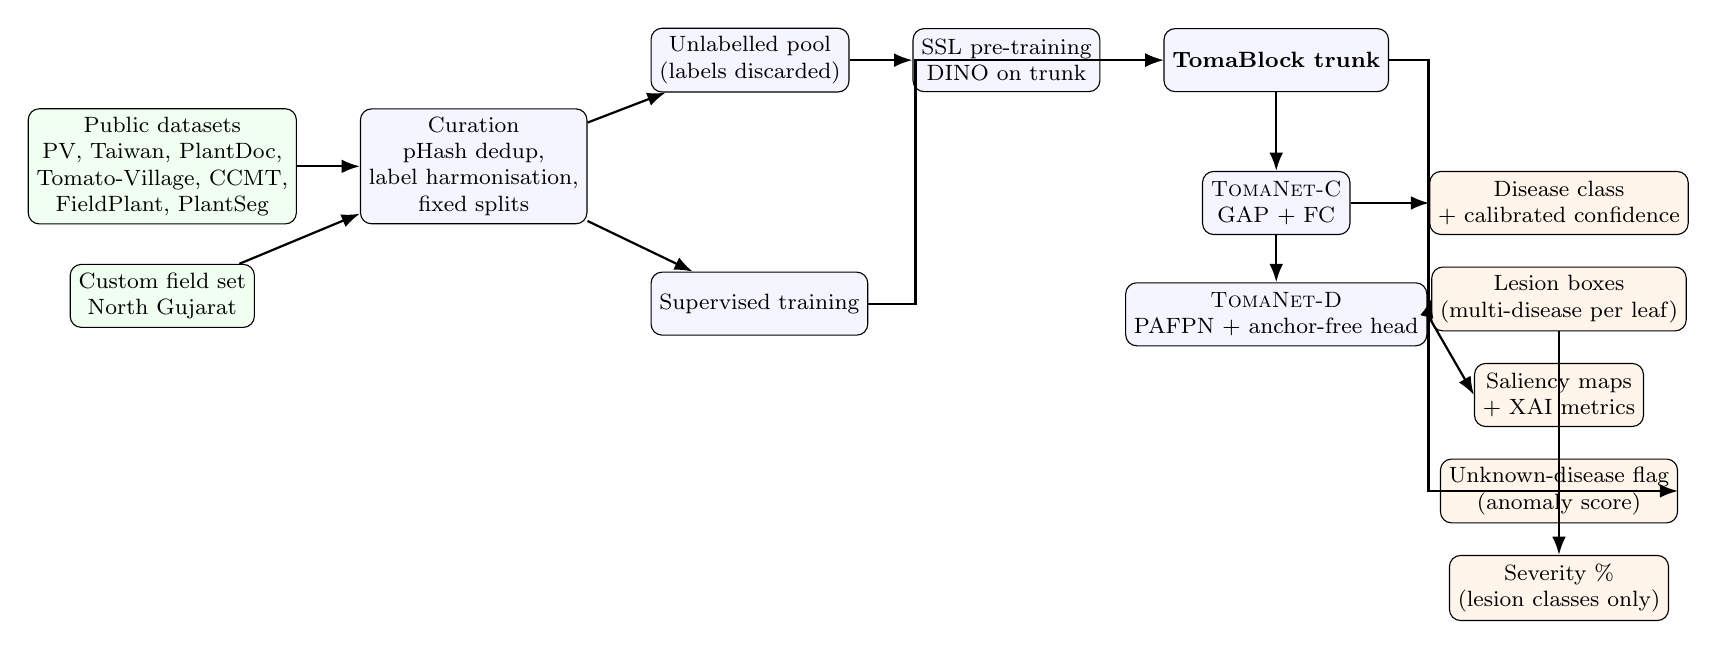
\begin{tikzpicture}[
  font=\footnotesize,
  box/.style={draw,rounded corners,align=center,minimum height=8mm,inner sep=3pt,fill=blue!4},
  dat/.style={draw,rounded corners,align=center,minimum height=8mm,inner sep=3pt,fill=green!6},
  res/.style={draw,rounded corners,align=center,minimum height=8mm,inner sep=3pt,fill=orange!8},
  ar/.style={-{Latex},thick}
]
\node[dat] (d1) {Public datasets\\PV, Taiwan, PlantDoc,\\Tomato-Village, CCMT,\\FieldPlant, PlantSeg};
\node[dat,below=5mm of d1] (d2) {Custom field set\\North Gujarat};
\node[box,right=8mm of d1] (pp) {Curation\\pHash dedup,\\label harmonisation,\\fixed splits};
\node[box,above right=2mm and 8mm of pp] (pool) {Unlabelled pool\\(labels discarded)};
\node[box,right=8mm of pool] (ssl) {SSL pre-training\\DINO on trunk};
\node[box,below right=6mm and 8mm of pp] (sup) {Supervised training};
\node[box,right=8mm of ssl] (trunk) {\textbf{TomaBlock trunk}};
\node[box,below=10mm of trunk] (cls) {\modelcls\\GAP + FC};
\node[box,below=6mm of cls] (det) {\modeldet\\PAFPN + anchor-free head};
\node[res,right=10mm of cls] (o1) {Disease class\\+ calibrated confidence};
\node[res,below=4mm of o1] (o2) {Lesion boxes\\(multi-disease per leaf)};
\node[res,below=4mm of o2] (o3) {Saliency maps\\+ XAI metrics};
\node[res,below=4mm of o3] (o4) {Unknown-disease flag\\(anomaly score)};
\node[res,below=4mm of o4] (o5) {Severity \%\\(lesion classes only)};
\draw[ar] (d1) -- (pp); \draw[ar] (d2) -- (pp);
\draw[ar] (pp) -- (pool); \draw[ar] (pp) -- (sup);
\draw[ar] (pool) -- (ssl); \draw[ar] (ssl) -- (trunk);
\draw[ar] (sup.east) -- ++(6mm,0) |- (trunk.west);
\draw[ar] (trunk) -- (cls); \draw[ar] (cls) -- (det);
\draw[ar] (cls) -- (o1); \draw[ar] (det.east) -- (o2.west);
\draw[ar] (det.east) -- (o3.west); \draw[ar] (trunk.east) -- ++(5mm,0) |- (o4.east);
\draw[ar] (o2) -- (o5);
\end{tikzpicture}
\end{center}

\subsection{Stage-by-stage}
\begin{description}[style=nextline]
  \item[S1 -- Curation.] Download from \emph{original} sources (GitHub/Mendeley/Zenodo), not Kaggle re-uploads, so licences and provenance are traceable. Perceptual-hash deduplication within and \emph{across} datasets (PlantVillage derivatives overlap heavily). Map every dataset's class names onto the canonical vocabulary (Table~\ref{tab:classes}). Emit fixed split files + a manifest with per-image SHA-256.
  \item[S2 -- Task-specific pre-processing.] \emph{Classification}: resize shorter side, random-resized-crop to 224 (256 variant for PlantVillage native), ImageNet normalisation, RandAugment + Mixup/CutMix. \emph{Detection}: letterbox to 640, mosaic + HSV + flips + scale, closed mosaic for the last 10 epochs. One-hot encoding is used only for the classifier; detection uses box labels (this corrects B8).
  \item[S3 -- Pre-training.] DINO on the unlabelled pool (\S\ref{sec:unsup}), producing trunk weights that both heads can load.
  \item[S4 -- Supervised training.] \modelcls{} and \modeldet{} from the shared trunk, plus all baselines under identical recipes.
  \item[S5 -- Inference.] Two deployment modes: (a) \emph{whole-image classification} for single-leaf/phone-macro use; (b) \emph{detection} for canopy images, which yields per-lesion boxes and therefore multi-disease-per-leaf output. Both emit a calibrated confidence (temperature scaling fitted on validation) and an anomaly score; if the anomaly score exceeds the threshold the prediction is returned as \emph{unknown} rather than forced into one of the 10 classes.
  \item[S6 -- Explanation and severity.] Saliency map for the predicted class/box, scored quantitatively (\S\ref{sec:metrics}); lesion-area ratio inside boxes for the four lesion-forming classes.
\end{description}

\subsection{Deliverables}
Code (fork of Ultralytics + a thin experiment runner), split manifests, trained weights, the North-Gujarat dataset with DOI, and one results script that regenerates every table in the paper from saved predictions -- so that no number is ever typed by hand (this is what prevents A1/B1 from recurring).

\section{Proposed Custom Model: \model}
\label{sec:model}

\subsection{Design requirements}
\begin{enumerate}
  \item One block definition (\textsc{TomaBlock}) reused, without modification, in the classifier trunk, the detector trunk \emph{and} the detector neck.
  \item Two architectures built from it: \modelcls{} (image classification, 224--256 px input) and \modeldet{} (object detection, 640 px input). Same stem and stage layout, so a trunk pre-trained for one task initialises the other.
  \item Budget: $\le 5$\,M parameters and $\le 10$ GFLOPs at 640 px for the ``n'' scale, so training fits on one 8--12\,GB GPU and inference runs on a phone / Jetson.
  \item Every architectural choice is justified by a small-lesion or field-image argument and gets an ablation row.
\end{enumerate}

\subsection{\textsc{TomaBlock}}
\label{sec:block}
Input $X\in\mathbb{R}^{C\times H\times W}$, expansion ratio $e{=}2$, partial ratio $r{=}1/4$.
\begin{align}
X_1 &= \mathrm{PConv}_{3\times3}(X;\, r) && \text{spatial mixing on $rC$ channels only (FasterNet)}\\
X_2 &= \sigma(\mathrm{BN}(\mathrm{Conv}_{1\times1}(X_1;\, C\!\to\! eC))) && \text{expand}\\
X_3 &= \mathrm{DWConv}_{k\times k}(X_2) \;\; (k{=}3 \text{ in stages 1--2},\, 5 \text{ in stages 3--4}) && \text{large-kernel context}\\
X_4 &= \mathrm{CA}(X_3) && \text{coordinate attention (H- and W-wise pooling)}\\
Y &= X + \mathrm{BN}(\mathrm{Conv}_{1\times1}(X_4;\, eC\!\to\! C)) && \text{project + residual}
\end{align}
with $\sigma=$ SiLU. At training time the $3\times3$ PConv has a parallel $1\times1$ branch and an identity branch (RepVGG style); the three are fused into a single $3\times3$ kernel for inference. Rationale:
\begin{itemize}
  \item \textbf{PConv} keeps FLOPs and \emph{memory access} low (the real bottleneck on edge devices), unlike depthwise-only designs.
  \item \textbf{Depthwise $5\times5$ in deep stages} gives lesion-scale receptive field growth without extra parameters (ConvNeXt finding).
  \item \textbf{Coordinate attention} encodes position along $H$ and $W$; lesions are small, position-specific, and easily lost by channel-only SE/ECA. CA is cheap ($\sim$2\% params).
  \item \textbf{Re-parameterisation} gives multi-branch training accuracy at single-branch inference cost.
\end{itemize}
A stage is $n_i$ \textsc{TomaBlock}s preceded by a stride-2 $3\times3$ conv (downsample). A \textsc{TomaStage}$(C_i, n_i)$ therefore has a single hyper-parameter pair per stage.

\subsection{Trunk (shared)}
\begin{center}
\begin{tabular}{@{}lccccc@{}}
\toprule
Scale & Stem ch. & $C_1..C_4$ & $n_1..n_4$ & Params (trunk, approx.) & Output strides \\
\midrule
n & 16 & 32, 64, 128, 256 & 1, 2, 2, 1 & $\approx$1.1\,M & 4, 8, 16, 32 \\
s & 32 & 64, 128, 256, 512 & 1, 2, 2, 1 & $\approx$4.3\,M & 4, 8, 16, 32 \\
m & 48 & 96, 192, 384, 576 & 2, 4, 4, 2 & $\approx$11\,M & 4, 8, 16, 32 \\
\bottomrule
\end{tabular}
\end{center}
Stem: two $3\times3$ stride-2 convs (like YOLOv8), i.e.\ stride 4 before stage~1. Parameter counts are estimates from the block formula and must be replaced by \texttt{thop}/\texttt{fvcore} measurements once implemented (\S\ref{sec:impl}).

\subsection{\modelcls{} -- classification architecture}
\[
\text{Stem} \to \text{S}_1 \to \text{S}_2 \to \text{S}_3 \to \text{S}_4 \to \mathrm{Conv}_{1\times1}(C_4\!\to\!1280) \to \mathrm{GAP} \to \mathrm{Dropout}(0.2) \to \mathrm{FC}(1280\!\to\!K)
\]
This is exactly the Ultralytics \texttt{Classify} head (\texttt{Conv(c1,1280,1)} $\to$ \texttt{AdaptiveAvgPool2d} $\to$ \texttt{Dropout} $\to$ \texttt{Linear}), so the YAML for \modelcls{} is the shared backbone list plus one \texttt{Classify} line -- the same pattern Ultralytics uses for \texttt{yolo11.yaml} vs.\ \texttt{yolo11-cls.yaml}, whose backbone lists are byte-identical.
Input 224 px for parity with ImageNet-pretrained baselines; 256 px variant for PlantVillage native resolution. $K=10$ (PlantVillage tomato) or dataset-specific. The $1\times1$ expansion before pooling follows MobileNetV3 and costs almost nothing at $7\times7$ resolution. Loss: cross-entropy with label smoothing 0.1; class-balanced (effective-number) weights when the imbalance ratio exceeds 5.

\subsection{\modeldet{} -- detection architecture}
\begin{itemize}
  \item \textbf{Backbone}: same stem + S$_1$..S$_4$; export P2 (stride 4), P3 (8), P4 (16), P5 (32). SPPF on P5.
  \item \textbf{Neck}: PAFPN (top-down + bottom-up) in which every fusion node is a \textsc{TomaBlock} (replacing YOLOv8's C2f). A \emph{P2 head is optional} and ablated: lesions on a 640-px field image are frequently $<16$ px, i.e.\ below one P3 cell.
  \item \textbf{Head}: anchor-free decoupled head (separate cls / reg branches) with Distribution Focal Loss (DFL, 16 bins) for box regression, exactly as in YOLOv8, so that Ultralytics' Task-Aligned Assigner and mAP evaluation can be reused unchanged.
  \item \textbf{Losses}: $\mathcal{L} = \lambda_{cls}\,\mathrm{BCE} + \lambda_{box}\,\mathcal{L}_{IoU} + \lambda_{dfl}\,\mathrm{DFL}$ with default weights $(0.5, 7.5, 1.5)$. $\mathcal{L}_{IoU}\in\{\text{CIoU},\text{WIoU-v3},\text{MPDIoU}\}$ is an ablation; recent small-object papers favour WIoU/MPDIoU; the plan starts from CIoU (the default) and only adopts an alternative if it wins on the validation split.
  \item \textbf{Post-processing}: standard NMS (IoU 0.7, conf 0.25 for reporting P/R/F1; conf 0.001 for mAP). Multi-label per leaf is handled natively: several boxes of different classes on one leaf. An NMS-free variant (YOLOv10-style dual assignment: one-to-many TAL top-$k{=}10$ + one-to-one top-$k{=}1$ head, \texttt{end2end=True} in the \texttt{Detect} head) is a cheap optional ablation because Ultralytics already implements it.
  \item \textbf{Loss caution}: recent agricultural papers report $+0.5$ to $+2$ mAP@0.5 from WIoU/MPDIoU/Inner-IoU/NWD, almost always single-dataset and single-seed -- within typical seed variance ($\approx$0.3--0.5 mAP). Only CIoU/DIoU/GIoU are switchable in Ultralytics; others require patching \texttt{BboxLoss.forward}. Ablate with $\ge3$ seeds before claiming anything.
\end{itemize}

\subsection{Weight-sharing and the transfer chain}
\label{sec:transfer_chain}
\begin{center}
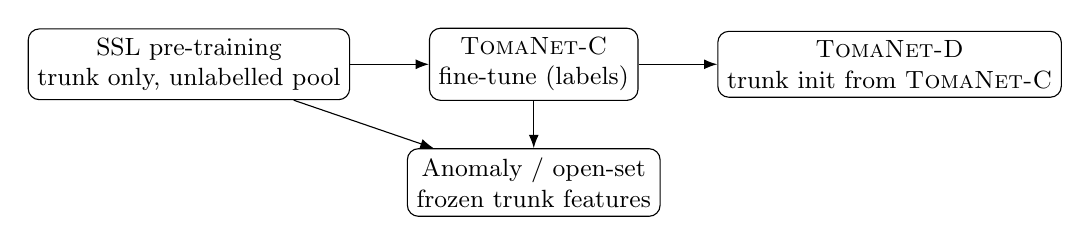
\begin{tikzpicture}[node distance=6mm and 10mm, every node/.style={draw,rounded corners,align=center,font=\small,minimum height=8mm}]
\node (ssl) {SSL pre-training\\ trunk only, unlabelled pool};
\node (cls) [right=of ssl] {\modelcls\\ fine-tune (labels)};
\node (det) [right=of cls] {\modeldet\\ trunk init from \modelcls};
\node (ano) [below=of cls] {Anomaly / open-set\\ frozen trunk features};
\draw[-{Latex}] (ssl) -- (cls);
\draw[-{Latex}] (cls) -- (det);
\draw[-{Latex}] (ssl) -- (ano);
\draw[-{Latex}] (cls) -- (ano);
\end{tikzpicture}
\end{center}
Three initialisations of the trunk are compared for both tasks: (a) random, (b) ImageNet-1k supervised (train \modelcls{} on ImageNet-1k for 100 epochs -- feasible at scale ``n'' in $\approx$2 GPU-days at 160 px; if not affordable, use ImageNet-100), (c) self-supervised on the pooled tomato images (\S\ref{sec:unsup}). This is the cleanest way to make the ``unsupervised'' track a measurable part of the main results rather than a side experiment.

\subsection{Implementation route}
\label{sec:impl}
Do not write a training loop. Both tasks are implemented inside \textbf{Ultralytics 8.x}, which already supports a \texttt{classify} task (\texttt{Classify} head with GAP + FC) and a \texttt{detect} task with the TAL assigner, DFL, mosaic augmentation, EMA, AMP, mAP evaluation and export (ONNX, TensorRT, TFLite).
\begin{enumerate}
  \item Implement \texttt{TomaBlock}, \texttt{TomaStage}, \texttt{CoordAtt}, \texttt{PConv} in one file \texttt{ultralytics/nn/modules/toma.py}. Ultralytics has \emph{no} plugin registry (a ``Python-in-YAML'' PR was closed on security grounds), so work on an editable fork (\texttt{pip install -e .}): export the classes in \texttt{nn/modules/\_\_init\_\_.py}, import them in \texttt{nn/tasks.py}, add them to the \texttt{base\_modules} set (so $c_1,c_2$ are injected with width scaling) and to \texttt{repeat\_modules} (so the YAML \texttt{repeats} column becomes $n$). Block signature must be \texttt{(c1, c2, *args)}.
  \item \texttt{tomanet-cls.yaml}: backbone list + \texttt{Classify} head. \texttt{tomanet-det.yaml}: same backbone list + SPPF + PAFPN of \texttt{TomaBlock} + \texttt{Detect} head. Scales \texttt{n/s/m} through the standard \texttt{scales:} dictionary (depth, width, max-channels).
  \item Verify with \texttt{model.info()} (params, GFLOPs) and one forward pass per task; unit test: fused vs unfused block outputs agree to $10^{-4}$.
  \item SSL pre-training uses the same trunk exported as a plain \texttt{nn.Module} into a Lightly / solo-learn DINO or MAE recipe; weights are loaded back with a key-mapping script.
  \item FLOPs/latency: \texttt{thop} for GFLOPs, \texttt{torch.utils.benchmark} for GPU latency, ONNX Runtime for CPU latency, TensorRT-FP16 on Jetson if hardware is available.
\end{enumerate}

\subsection{Ablation list (one row each)}
\begin{enumerate}[label=Abl-\arabic*]
  \item Full block vs.\ block without CA vs.\ CA replaced by SE / ECA / CBAM.
  \item PConv vs.\ full $3\times3$ conv vs.\ depthwise-only.
  \item Rep-branch on/off.
  \item $k=5$ in deep stages vs.\ $k=3$ everywhere.
  \item Detector: with vs.\ without P2 head; \textsc{TomaBlock} neck vs.\ C2f neck.
  \item Loss: CIoU vs.\ WIoU-v3 vs.\ MPDIoU.
  \item Trunk init: scratch vs.\ ImageNet vs.\ SSL (tomato pool).
  \item Input resolution: 224 vs.\ 256 (cls); 640 vs.\ 800 (det).
\end{enumerate}

\section{Unsupervised and Self-Supervised Track}
\label{sec:unsup}

\subsection{Direct answer: is unsupervised learning suitable here?}
Partly. The evidence from 2021--2026 splits cleanly into four verdicts.

\begin{center}\small
\begin{tabular}{@{}L{3.4cm}L{1.7cm}L{10.2cm}@{}}
\toprule
Approach & Verdict & Evidence \\
\midrule
Self-supervised \emph{pre-training}, then fine-tune with few labels & \textbf{Use it} & Domain SSL on only 3\,000 unlabelled agricultural images beats ImageNet-21k supervised transfer ($+7.90$ vs $+5.55$ over random init); gain grows with pool size: 500 imgs $+1.56$, 1k $+2.78$, 2k $+4.00$, 3k $+4.57$~\cite{sonavane2026}. PlantCLR (SimCLR + ConvNeXt-T) 99.10\% PV / 96.83\% field cassava~\cite{plantclr}. Frozen DINOv2 linear probe $\approx$97\% on leaf disease, consistently $>$ ImageNet-1k pre-training~\cite{espejo2025}. \\
Healthy-only \emph{anomaly detection} for unknown disease & \textbf{Use it} & Colour-reconstructability (pix2pix + CIEDE2000) AUROC \textbf{0.99} on PV potato trained on 76 healthy leaves; AnoGAN 0.97, OC-SVM 0.95, AE-SSIM 0.94~\cite{katafuchi2021}. VQ-VAE 0.983 (cherry) / 0.936 (pepper)~\cite{calabro2022}. Healthy-ID vs diseased-OOD on PV: AUROC 99.6--99.85, FPR95 0.71--1.68~\cite{dong2025}. \\
Semi-supervised (pseudo-label, Mean Teacher, FixMatch) & \textbf{Use it, modestly} & Mean Teacher 88.50\% with \textbf{5\%} labels on 38-class PV~\cite{ilsever2024}; AaSSL $+1.7$ to $+3.4$\,pp over supervised at 5--20\% labels, $<1$\,pp at $\ge$50\%~\cite{aassl2025}. On tomato specifically only one weak result exists: TOM-SSL 72.51\% at 10\% labels (PV-tomato), 70.87\% (Taiwan)~\cite{tomssl2025} -- a low bar. \\
Unsupervised \emph{clustering} to recover disease classes & \textbf{Do not} & Raw ResNet-50 $k$-means on PV apple+grape (8 classes): NMI 0.272, purity 0.396. The best specialised method (CIKICS) reaches NMI 0.636 / purity 0.683 / F1 0.835~\cite{cikics}; on citrus only NMI 0.331. Clusters follow species, colour and lighting, not pathology; early blight / Septoria / target spot merge. Use clustering only for pre-annotation and active-learning proposals. \\
Fully unsupervised domain adaptation lab$\to$field & \textbf{Not alone} & Tomato is the \emph{worst} target in the UDA literature: MSUN reaches 50.58\% on tomato (vs 96.78\% on corn), from a 41.81\% source-only baseline~\cite{msun2023}. Ten labelled field images per disease with metric-based few-shot DA gives $+11.1$ to $+29.3$ F1~\cite{fmda2024} -- far better than any unsupervised method. CycleGAN field$\to$lab translation reaches F1 95.6 but only by translating field images into lab style at inference~\cite{cho2023}. \\
\bottomrule
\end{tabular}
\end{center}

\subsection{What the literature has \emph{not} done on tomato (the openings)}
These are verified absences, each cheap to fill and each a defensible contribution:
\begin{enumerate}[label=U\arabic*]
  \item \label{u1} \textbf{No label-efficiency curve for any SSL method on tomato.} Every plant-SSL paper found fine-tunes with 100\% of labels. A 1/5/10/25/100\% curve on PV-tomato \emph{and} on field tomato, with SSL vs ImageNet vs scratch, does not exist.
  \item \label{u2} \textbf{No modern anomaly-detection benchmark on tomato.} PatchCore, PaDiM, SimpleNet, DRAEM and reverse distillation have never been reported on tomato healthy$\to$diseased. Only potato (0.99) and cherry/pepper (0.98/0.94) exist.
  \item \label{u3} \textbf{No NMI/ARI/purity on the 10-class PV-tomato subset.} CIKICS covered apple/grape/peach/strawberry/citrus; the one tomato clustering paper used 300 images, 3 classes, and reported only internal indices (silhouette 0.273)~\cite{wdmtsne}.
  \item \label{u4} \textbf{No leave-one-disease-out open-set benchmark on tomato.} Existing tomato OOD work is the easy setting (healthy = in-distribution, any disease = OOD) or open-vocabulary detection~\cite{pdcvld}. ``9 diseases known, 1 held out'' with AUROC/FPR95 is unreported.
  \item \label{u5} \textbf{No frozen DINOv2/v3 $k$-NN or linear-probe number on tomato}, despite it being the cheapest possible baseline.
  \item \label{u6} \textbf{Unsupervised lesion-ratio severity on tomato is never validated against expert scores} with concordance $\rho_c$ or $R^2$, although tomato severity ground truth exists (bacterial spot, 150 leaves, raters $\rho_c$ 0.83$\to$0.96 with standard area diagrams~\cite{sad2015}).
\end{enumerate}

\subsection{Track U1 -- Self-supervised pre-training (feeds E4)}
\begin{itemize}
  \item \textbf{Pool}: union of all training images from every dataset in \S\ref{sec:datasets} plus unannotated Custom images, labels discarded ($\approx$40--60k images). Test images excluded by hash.
  \item \textbf{Method}: DINO (multi-crop $2\times224 + 6\times96$, teacher momentum $0.996\to1$, 300 epochs) on the \model{} trunk. Fallback if compute-bound: SimCLR/MoCo-v3, 200 epochs. Note that~\cite{sonavane2026} obtained $+4.57$\,pp from only 3\,000 images, so the pool size here is comfortable.
  \item \textbf{Evaluation}: $k$-NN ($k{=}20$, cosine, $T{=}0.07$) and linear probe on frozen features, then the label-efficiency curve of~\ref{u1} at 1/5/10/25/100\% labels $\times$ 3 seeds, for \emph{both} classification and detection (detection uses the SSL trunk as initialisation).
  \item \textbf{Reference points to beat}: TOM-SSL 72.51\% at 10\% labels on PV-tomato~\cite{tomssl2025}; Mean Teacher 88.50\% at 5\% labels on 38-class PV~\cite{ilsever2024}; frozen DINOv2 linear probe (run it -- it is one afternoon of compute and currently unpublished for tomato,~\ref{u5}).
\end{itemize}

\subsection{Track U2 -- Unknown-disease flagging (feeds E5)}
Two settings, both trained \emph{without} labels for the target condition:
\begin{enumerate}
  \item \textbf{Healthy-only anomaly detection.} Memory-bank (PatchCore) over frozen \model{} trunk features of healthy leaves only; score = distance to the bank. Compare against PaDiM, an autoencoder and the colour-reconstructability baseline~\cite{katafuchi2021}. Report image-level AUROC/AUPR/FPR95 on lab images \emph{and} on field images -- the expected result is a large drop on field backgrounds (pepper already shows 0.936 vs cherry 0.983), and documenting that drop is itself the finding.
  \item \textbf{Leave-one-disease-out open set} (\ref{u4}). Train on 9 classes, hold out 1; score with (a) max-softmax, (b) energy, (c) PatchCore distance, (d) Mahalanobis on trunk features. Rotate the held-out class over all 10; report mean AUROC/FPR95 per held-out disease. Expect max-softmax to be weak -- OpenMax reached only 0.812 AUROC / 70.1\% accuracy on strawberry, while outlier-exposure and energy/VPT tuning reached 0.972 and 94--98~\cite{openmatch2022,dong2024}.
\end{enumerate}

\subsection{Track U3 -- Severity as lesion-area ratio (scoped)}
Inside each predicted box: SAM-2 (prompted with the box) for the leaf mask, then $k$-means in Lab colour space \emph{inside} the mask for lesion pixels; severity $= |\text{lesion}| / |\text{leaf}|$. Validate against the 300-image polygon subset (Pearson $r$, MAE) and, if an agronomist can score them, against ordinal severity classes (weighted $\kappa$), which would close~\ref{u6}. Two documented cautions: vanilla SAM is poor at \emph{lesions} directly (adapters add $+41$ Dice~\cite{samadapter}; zero-shot leaf recall 63.2 vs 78.7 for trained Mask R-CNN~\cite{leafonlysam}), so SAM is used for the \emph{leaf} mask only; and colour-ratio severity is meaningless for TYLCV, mosaic and mite damage, which have no discrete lesions -- severity is therefore reported only for the four lesion-forming classes (early blight, late blight, Septoria, target spot) and explicitly declared not applicable elsewhere.

\subsection{What is deliberately \emph{not} attempted}
Fully unsupervised lab$\to$field adaptation as a headline result (best published tomato number is 50.58\%); clustering as a substitute for labels; unsupervised discovery of new disease \emph{classes} (only flagging that something is unknown). These are stated as limitations rather than quietly omitted.

\section{Baselines and Comparative Models}
\label{sec:baselines}

Every model that appears in the literature survey of the slides is included, plus the current (2025--2026) state of the art; otherwise the comparison is dated. All baselines are trained on the \emph{same} splits with the \emph{same} recipe family (\S\ref{sec:experiments}) and reported with params, GFLOPs and latency. Parameter/FLOP figures below are the standard published values (ImageNet, 224 px for classifiers; 640 px for detectors) and are re-measured with \texttt{thop} in the final tables. \textbf{Convention:} Ultralytics reports GFLOPs $=2\times$MACs at 640 px; \texttt{thop}/\texttt{ptflops} return MACs; \texttt{fvcore} counts 1 MAC as 1 FLOP. The final tables state one convention and re-measure every model with the same tool. Detector mAP context on COCO (n-scale): YOLOv8n 37.3, YOLOv10n 39.5, YOLO11n 39.5, YOLOv12n 40.6, YOLO26n 40.9.

\begin{longtable}{@{}L{3.6cm}L{1.6cm}L{1.6cm}L{1.6cm}L{6.6cm}@{}}
\caption{Classification baselines.}\label{tab:cls_baselines}\\
\toprule
Model & Params (M) & GFLOPs & In slides? & Role \\
\midrule
\endfirsthead
\toprule
Model & Params (M) & GFLOPs & In slides? & Role \\
\midrule
\endhead
\bottomrule
\endfoot
AlexNet & 61 & 0.7 & yes & historical; Chen 2022 (modified AlexNet) \\
VGG16 & 138 & 15.5 & yes & historical; Younis 2022, Nawaz 2023 \\
ResNet50 & 25.6 & 4.1 & yes & standard CNN reference \\
DenseNet121 & 8.0 & 2.9 & yes & the model in Deck A; Abbas 2021 (C-GAN + DenseNet121) \\
InceptionV3 & 23.8 & 5.7 & yes & Hosen 2025 \\
EfficientNet-B3 & 12.2 & 1.9 & yes & Ullah 2023 (EffiMob-Net), Ahmad 2021 \\
MobileNetV2 & 3.5 & 0.3 & yes & Sohib 2022; lightweight reference \\
MobileNetV3-Large & 5.4 & 0.22 & no & modern lightweight reference \\
SqueezeNet 1.1 & 1.2 & 0.35 & yes & Thuseethan 2022 (Siamese), Guha Paul 2023 \\
EfficientNetV2-S & 21.5 & 8.4 & no & strong modern CNN \\
ConvNeXt-Tiny & 28.6 & 4.5 & no & modern CNN; same design family as \model{} (large-kernel DW) \\
ViT-B/16 & 86 & 17.6 & yes & Gangwar 2023; transformer reference \\
Swin-Tiny & 28.3 & 4.5 & no & hierarchical transformer reference \\
MobileViT-S / EfficientViT-M2 & 5.6 / 4.2 & 2.0 / 0.2 & no & hybrid lightweight; Thai 2025 (CNN+Transformer) \\
YOLOv8n-cls / YOLO11n-cls / YOLO26n-cls & 2.7 / 1.6 / 2.8 & 0.5 / 0.5 / 0.5 (224 px) & no & same framework as \modelcls{}; fairest lightweight comparison (ImageNet top-1 $\approx$ 69 / 70 / 71.4) \\
RepViT-M0.9 / FastViT-T8 / StarNet-S1 & 5.1 / 3.6 / 2.9 & 0.8 / 0.7 / 0.4 & no & 2023--2024 mobile SOTA; closest competitors to \model{} by design \\
\textbf{\modelcls{}-n/s} & target 1.3 / 4.6 & target 0.3 / 1.0 & -- & proposed \\
\end{longtable}

\begin{longtable}{@{}L{3.6cm}L{1.6cm}L{1.6cm}L{1.6cm}L{6.6cm}@{}}
\caption{Detection baselines (640 px).}\label{tab:det_baselines}\\
\toprule
Model & Params (M) & GFLOPs & In slides? & Role \\
\midrule
\endfirsthead
\toprule
Model & Params (M) & GFLOPs & In slides? & Role \\
\midrule
\endhead
\bottomrule
\endfoot
Faster R-CNN R50-FPN & 41.5 & $\approx$180 & yes & two-stage reference (Deck B) \\
Mask R-CNN R50-FPN & 44 & $\approx$260 & yes & Junare 2025; only if masks exist \\
YOLOv4 / YOLOv4-tiny & 64 / 6 & 60 / 7 & yes & Wang 2021, Gangwar 2023 \\
YOLOv5s / YOLOv5n & 7.2 / 1.9 & 16.5 / 4.5 & yes & Oni 2025 \\
YOLOv8n / s & 3.2 / 11.2 & 8.7 / 28.6 & yes & Deck B model; Wang 2023 \\
YOLOv10n / s & 2.3 / 7.2 & 6.7 / 21.6 & no & NMS-free \\
YOLO11n / s & 2.6 / 9.4 & 6.5 / 21.5 & no & current Ultralytics default \\
YOLOv12n / s & 2.6 / 9.3 & 7.6 / 23.7 & no & attention-centric (area attention), Feb 2025 \\
YOLO26n / s & 2.4 / 9.5 & 5.4 / 20.7 & no & Jan 2026: NMS-free end-to-end, DFL removed, small-target-aware assignment (STAL) \\
RT-DETR-R18 & 20 & 60 & no & transformer detector reference \\
\textbf{\modeldet{}-n/s} & target 2.5 / 8 & target 7 / 22 & -- & proposed \\
\end{longtable}

\paragraph{Fairness rules.} (i) identical train/val/test image lists (hashes published); (ii) identical input resolution per task; (iii) identical epochs and early-stopping rule; (iv) baseline hyper-parameters left at their official defaults (Ultralytics for detectors, \texttt{timm} recipe for classifiers) -- tuning only \model{} would bias the comparison; (v) 3--5 seeds per model, mean$\pm$std; (vi) ImageNet initialisation for all baselines that have it, and both ImageNet and SSL initialisation for \model{} so the effect of pre-training is isolated from the effect of architecture.

\section{Evaluation Metrics}
\label{sec:metrics}
All metrics are computed by \texttt{torchmetrics} / \texttt{pycocotools} / Ultralytics validators from saved predictions; no hand-computed numbers. Notation: $K$ classes, $N$ test images, confusion matrix $M_{ij}$ (true $i$, predicted $j$), $\mathrm{TP}_k, \mathrm{FP}_k, \mathrm{FN}_k$ per class.

\subsection{Classification}
\begin{align}
\text{Accuracy} &= \tfrac{1}{N}\textstyle\sum_k M_{kk} \\
P_k = \tfrac{\mathrm{TP}_k}{\mathrm{TP}_k+\mathrm{FP}_k},\quad R_k &= \tfrac{\mathrm{TP}_k}{\mathrm{TP}_k+\mathrm{FN}_k},\quad F1_k = \tfrac{2P_kR_k}{P_k+R_k} \\
\text{Macro-}F1 &= \tfrac{1}{K}\textstyle\sum_k F1_k \qquad\text{(primary metric; robust to imbalance)}\\
\kappa &= \frac{p_o - p_e}{1-p_e},\quad p_o=\text{Accuracy},\ p_e = \textstyle\sum_k \tfrac{(\sum_j M_{kj})(\sum_i M_{ik})}{N^2}\\
\text{MCC} &= \frac{N\sum_k M_{kk} - \sum_k t_k p_k}{\sqrt{(N^2-\sum_k p_k^2)(N^2-\sum_k t_k^2)}},\ t_k=\textstyle\sum_j M_{kj},\ p_k=\textstyle\sum_i M_{ik}\\
\text{ECE} &= \textstyle\sum_{b=1}^{B} \tfrac{|S_b|}{N}\,\big|\mathrm{acc}(S_b)-\mathrm{conf}(S_b)\big| \quad (B=15 \text{ bins})
\end{align}
Also: per-class AUROC (one-vs-rest), top-2 accuracy (relevant for visually confusable pairs such as early vs.\ late blight), full confusion matrix in the appendix. Report \textbf{in-domain} (same dataset) and \textbf{cross-domain} (train on A, test on B) values; the \emph{generalisation gap} $\Delta = \text{Acc}_{\text{in}} - \text{Acc}_{\text{cross}}$ is a headline number.

\subsection{Detection}
COCO protocol via \texttt{pycocotools}:
\begin{align}
\text{IoU}(b,\hat b) &= \tfrac{|b\cap \hat b|}{|b\cup \hat b|} \\
\mathrm{AP}_k(\tau) &= \int_0^1 p_k(r;\tau)\,dr \quad \text{(101-point interpolation)},\\
\text{mAP@0.5} &= \tfrac1K\textstyle\sum_k \mathrm{AP}_k(0.5),\qquad
\text{mAP@[0.5{:}0.95]} = \tfrac1K\textstyle\sum_k \tfrac{1}{10}\sum_{\tau\in\{0.5,\dots,0.95\}} \mathrm{AP}_k(\tau)
\end{align}
plus AP$_s$/AP$_m$/AP$_l$ (area $<32^2$, $32^2$--$96^2$, $>96^2$ px -- lesions are mostly ``small''), AR@100, and P/R/F1 at conf 0.25 / IoU 0.5 for the deployment operating point. Primary metric: \textbf{mAP@[0.5:0.95]}; secondary: \textbf{AP$_s$}.

\subsection{Efficiency}
Params (M), GFLOPs at task resolution (\texttt{thop}), model size (MB, FP16 ONNX), latency (ms, batch 1, median of 200 runs after 20 warm-up) on: GPU (FP16), CPU (ONNX Runtime, 4 threads), and an edge device if available (Jetson Orin Nano / Raspberry Pi 5 / Android via TFLite). Report FPS $=1000/\text{latency}$. Optional: energy per image (Jetson \texttt{tegrastats}).

\subsection{Robustness}
\begin{itemize}
  \item \textbf{Cross-dataset matrix}: train on each of $\{$PlantVillage, Taiwan, Tomato-Village, Custom$\}$, test on all others; report macro-F1 (cls) / mAP@0.5 (det).
  \item \textbf{Corruption robustness} (ImageNet-C style, severities 1--5): Gaussian noise, motion blur, brightness, contrast, JPEG, fog; report mean corruption error relative to clean.
  \item \textbf{Background swap test}: PlantVillage leaves segmented (Otsu/SAM) and pasted on field backgrounds; accuracy drop quantifies background reliance.
\end{itemize}

\subsection{Explainability (quantitative)}
Given a saliency map $S\in[0,1]^{H\times W}$ and a ground-truth lesion mask $G$ (or the GT box when no mask exists -- state which):
\begin{align}
\text{Pointing game} &= \tfrac{1}{N}\textstyle\sum_n \mathbb{1}\big[\arg\max S_n \in G_n\big] \\
\text{Energy-based PG} &= \frac{\sum_{(i,j)\in G} S_{ij}}{\sum_{(i,j)} S_{ij}} \quad\text{(fraction of saliency mass inside the lesion)}\\
\text{Saliency IoU}(\theta) &= \tfrac{|\{S>\theta\}\cap G|}{|\{S>\theta\}\cup G|},\ \theta \text{ chosen so that } |\{S>\theta\}| = |G| \\
\text{Deletion / Insertion AUC} & \text{ (RISE protocol): remove / insert pixels in order of saliency; AUC of score-vs-fraction curve}
\end{align}
Methods compared: Grad-CAM, Grad-CAM++, Score-CAM, LayerCAM (classifier, last stage) and EigenCAM / Grad-CAM on P3--P4 neck features for the detector (target = class score of the matched box, computed before NMS). Sanity check: model-parameter randomisation test (Adebayo et al.) -- saliency must degrade when weights are randomised. ``NSR'' from Deck~B is dropped unless it can be defined.

\subsection{Unsupervised / self-supervised}
\begin{itemize}
  \item \textbf{SSL pre-training quality}: $k$-NN accuracy ($k{=}20$) and linear-probe accuracy on frozen features; label-efficiency curve: fine-tune with 1\%, 5\%, 10\%, 25\%, 100\% of labels (3 seeds each).
  \item \textbf{Anomaly / unknown-disease detection}: image-level AUROC and AUPR, and FPR@95\%TPR, for healthy vs.\ diseased and for known-vs-unknown (hold out 2 disease classes at train time).
  \item \textbf{Clustering}: NMI, ARI, purity of $k$-means ($k{=}K$) on frozen embeddings vs.\ true labels; silhouette score.
  \item \textbf{Severity (if lesion masks exist)}: Pearson $r$ and MAE between predicted lesion-area ratio and annotated ratio; agreement with ordinal severity classes via weighted kappa.
\end{itemize}

\subsection{Statistics}
Every table cell = mean$\pm$std over $\ge 3$ seeds (5 for headline models). Model-vs-model differences tested with McNemar (classification, paired on the same test images) or a paired $t$-test over seeds (mAP); report $p$-values for the headline claims. Publish the exact split files (image hashes) with the code.

\section{Experimental Plan}
\label{sec:experiments}

\subsection{Gap-to-experiment mapping}
\begin{table}[H]
\centering\small
\caption{Every gap claimed in the research-gap slide is tied to a measurable experiment or explicitly dropped.}\label{tab:gap_map}
\begin{tabular}{@{}L{4.6cm}L{6.2cm}L{4.4cm}@{}}
\toprule
Claimed gap & Experiment in this plan & Metric \\
\midrule
Lab-only data; accuracy drop in the field & E3 cross-dataset matrix; background-swap test & $\Delta$ macro-F1, mAP gap \\
Class imbalance & class-balanced loss + resampling ablation on Tomato-Village and Custom & macro-F1 vs accuracy gap, per-class F1 \\
Multiple diseases on one leaf & detection on Tomato-Village / Custom (multi-box, multi-class) & per-image multi-label F1 \\
No lesion localisation & \modeldet{} boxes; saliency IoU & mAP, AP$_s$, saliency IoU \\
Severity not measured & scoped: lesion-area ratio inside boxes via SAM / colour clustering on a 300-image mask subset & Pearson $r$, MAE \\
Unknown / unseen disease & E5 anomaly + open-set (hold out 2 classes) & AUROC, FPR@95 \\
Explainability qualitative only & E6 quantitative XAI & PG, energy-PG, deletion AUC \\
Fruit ``disease'' & scoped to ripeness / maturity detection on LaboroTomato + Kaggle fruit; disorders only if annotated & mAP \\
Temporal progression & \textbf{dropped} -- no time-series data & -- \\
Pests & only if the Custom set contains annotated pest classes & mAP \\
\bottomrule
\end{tabular}
\end{table}

\subsection{Data protocol}
\label{sec:data_protocol}
\begin{enumerate}
  \item \textbf{Deduplicate} every dataset with perceptual hashing (pHash, Hamming $\le 6$); PlantVillage and its Kaggle derivatives contain near-duplicates and augmented copies, which leak across splits. Report how many were removed.
  \item \textbf{Splits}: stratified 70/15/15 (train/val/test) per dataset, fixed by seed 0, released as file lists. Model selection on val only; test touched once per final model.
  \item \textbf{Label harmonisation}: one canonical tomato class vocabulary (Table~\ref{tab:classes}) with a mapping from every dataset's class names; classes absent from a dataset are marked so cross-dataset tests only score shared classes.
  \item \textbf{Unlabelled pool} for SSL: union of all training images of all datasets plus unannotated Custom images, labels discarded. No test image may enter the pool.
\end{enumerate}

\begin{table}[H]
\centering\small
\caption{Canonical class vocabulary (tomato leaf). Extend as datasets require.}\label{tab:classes}
\begin{tabular}{@{}llll@{}}
\toprule
ID & Canonical class & Pathogen type & Typical lesion size \\
\midrule
0 & Healthy & -- & -- \\
1 & Bacterial spot (\emph{Xanthomonas} spp.) & bacterial & small (1--3 mm) \\
2 & Early blight (\emph{Alternaria solani}) & fungal & medium, concentric rings \\
3 & Late blight (\emph{Phytophthora infestans}) & oomycete & large, water-soaked \\
4 & Leaf mold (\emph{Passalora fulva}) & fungal & diffuse, underside \\
5 & Septoria leaf spot & fungal & small, many \\
6 & Two-spotted spider mite & pest damage & stippling, whole-leaf \\
7 & Target spot (\emph{Corynespora}) & fungal & medium, bullseye \\
8 & Yellow leaf curl virus (TYLCV) & viral & whole-leaf (curl, yellowing) \\
9 & Mosaic virus (ToMV) & viral & whole-leaf mottling \\
10+ & Powdery mildew, leaf miner, nutrient deficiency, \dots & as present in field sets & -- \\
\bottomrule
\end{tabular}
\end{table}

\subsection{Custom North-Gujarat dataset: what to do with it}
\label{sec:custom_dataset}
This is the project's most valuable asset. Minimum documentation for publication (dataset card): location and dates, crop variety, growth stage, camera/phone models, distance and lighting, number of plants/fields, class list with agronomist confirmation, annotation tool (CVAT / Label Studio / Roboflow), annotation protocol (box around each lesion cluster vs.\ whole leaf), number of annotators and inter-annotator agreement (box IoU $\ge 0.5$ agreement rate, Cohen's $\kappa$ for class), split lists, licence (CC BY 4.0). Target: all 3\,153 images with image-level labels; $\ge 1\,500$ with boxes; $\ge 300$ with lesion polygons (for severity and XAI). Release on Zenodo with a DOI; cite it as a contribution.

\subsection{Experiments}
\begin{description}[style=nextline]
  \item[E1 -- In-domain classification.] All Table~\ref{tab:cls_baselines} models + \modelcls{} on PlantVillage-tomato, Taiwan, Tomato-Village (cls split), Custom. 5 seeds. Expected outcome: everything $\ge 99\%$ on PlantVillage (saturated); differences appear on field sets.
  \item[E2 -- In-domain detection.] Table~\ref{tab:det_baselines} models + \modeldet{} on Tomato-Village (det), PlantDoc-tomato boxes, Custom. 3 seeds. Report AP$_s$ separately.
  \item[E3 -- Cross-domain.] Train on $X$, test on $Y$ for all dataset pairs; both tasks. The key figure of the paper is the heat-map of generalisation gaps, with \model{} vs.\ the best baseline.
  \item[E4 -- Label efficiency / SSL.] Trunk pre-trained by DINO (or MAE) on the unlabelled pool; fine-tune with 1/5/10/25/100\% labels; compare to ImageNet init and scratch. Both tasks.
  \item[E5 -- Unknown-disease flagging.] Hold out 2 classes (e.g.\ target spot, mosaic) from training; PatchCore-style memory bank on frozen trunk features of healthy + known classes; AUROC for detecting held-out classes at test time. Compare with max-softmax, energy score, and a plain healthy-only autoencoder.
  \item[E6 -- Quantitative XAI.] Saliency metrics of \S\ref{sec:metrics} on the lesion-mask subset for \modelcls{}, \modeldet{}, DenseNet121, YOLOv8. Sanity check with randomised weights.
  \item[E7 -- Efficiency.] Latency/FPS/size on GPU, CPU, and one edge device; accuracy-vs-latency Pareto plot with all models.
  \item[E8 -- Ablations.] Abl-1..8 from \S\ref{sec:model}, on Tomato-Village (det) and Taiwan (cls), 3 seeds.
\end{description}

\subsection{Training recipes (fixed across models)}
\begin{itemize}
  \item \textbf{Classification} (\texttt{timm}-style): AdamW, lr $1\times10^{-3}\times\frac{\text{batch}}{256}$ , weight decay 0.05, cosine schedule, 5 warm-up epochs, 100 epochs, label smoothing 0.1, RandAugment (m9,n2), Mixup 0.2 / CutMix 1.0, random-resized-crop (scale 0.35--1), horizontal + vertical flip, colour jitter 0.3, EMA 0.9998, AMP, batch 64--128 at 224 px. Early stop on val macro-F1, patience 15.
  \item \textbf{Detection} (Ultralytics defaults): SGD lr0 0.01, momentum 0.937, wd $5\times10^{-4}$, warm-up 3 epochs, cosine, 200 epochs, mosaic 1.0 (closed for the last 10 epochs), mixup 0.1, HSV jitter, flips, scale 0.5, imgsz 640, batch 16--32, EMA, AMP. Early stop on val mAP@[0.5:0.95], patience 30.
  \item \textbf{SSL} (DINO, ViT-free version on the CNN trunk, as in solo-learn): 300 epochs on the pool, multi-crop $2\times224 + 6\times96$, AdamW, batch 128, teacher momentum 0.996$\to$1. Alternative if compute-bound: MoCo-v3 / SimCLR 200 epochs.
\end{itemize}

\subsection{Compute budget (single 12\,GB GPU, e.g.\ RTX 3060/4070)}
\begin{center}\small
\begin{tabular}{@{}lrrr@{}}
\toprule
Item & Runs & GPU-h / run (approx.) & Total GPU-h \\
\midrule
E1 classification: 16 models $\times$ 4 datasets $\times$ 5 seeds & 320 & 0.5--1.5 & $\approx$300 \\
E2 detection: 12 models $\times$ 3 datasets $\times$ 3 seeds & 108 & 2--6 & $\approx$400 \\
E3 cross-domain (evaluation only) & -- & -- & $\approx$10 \\
E4 SSL pre-training + 5 label fractions $\times$ 2 tasks $\times$ 3 seeds & 1 + 30 & 40 + 1 & $\approx$80 \\
E5 anomaly (feature extraction + memory bank) & 10 & 0.5 & 5 \\
E6 XAI & -- & -- & 5 \\
E8 ablations: 8 $\times$ 2 tasks $\times$ 3 seeds & 48 & 1--4 & $\approx$120 \\
\midrule
\multicolumn{3}{@{}l}{\textbf{Total}} & $\approx$900 GPU-h $\approx$ 6 weeks of continuous single-GPU time \\
\bottomrule
\end{tabular}
\end{center}
If this is too much, cut seeds to 3 for E1/E2 and drop the ``m'' scale; that halves it.

\subsection{Timeline (indicative)}
\begin{enumerate}
  \item Weeks 1--2: download, deduplicate, harmonise labels, publish split files; write dataset card and start box annotation of the Custom set.
  \item Weeks 3--4: implement \textsc{TomaBlock} + both YAMLs in Ultralytics; unit tests; param/FLOP table.
  \item Weeks 5--8: E1, E2 (baselines run in the background while annotation continues).
  \item Weeks 9--10: E4 SSL pre-training and label-efficiency.
  \item Weeks 11--12: E3, E5, E6, E7, E8.
  \item Weeks 13--14: figures, statistics, writing; dataset release.
\end{enumerate}

\section{Risks and Mitigations}
\label{sec:risks}
\begin{tabular}{@{}L{5.2cm}L{10.8cm}@{}}
\toprule
Risk & Mitigation \\
\midrule
\model{} does not beat YOLO11/12 or ConvNeXt in-domain. & Likely on PlantVillage (saturated). The paper's claim is \emph{Pareto} (accuracy at $\le 3$\,M params) and \emph{cross-domain} robustness, not in-domain SOTA. Frame it that way from the start. \\
Custom-set annotation is slow / inconsistent. & Start now; annotate boxes only for lesion clusters; use YOLOv8 pre-labels + human correction in CVAT; measure agreement on a 100-image overlap. \\
SSL gives no gain over ImageNet init. & Report it honestly -- a negative label-efficiency result on a 50k-image pool is itself informative; the anomaly-detection track still uses the features. \\
Grad-CAM metrics need masks that do not exist. & 300 polygon annotations $\approx$ 2 person-days; alternatively use PlantSeg tomato masks if licence permits. \\
Compute. & Scale ``n'' only for baselines-vs-ours full grid; ``s'' only for headline datasets. \\
Public datasets have licence restrictions (e.g.\ Kaggle re-uploads without licence). & Use original sources (PlantVillage GitHub / Mendeley / Zenodo); record licence per dataset in the card. \\
\bottomrule
\end{tabular}

\begin{thebibliography}{99}
\footnotesize
\bibitem{mohanty2016} S.~P. Mohanty, D.~P. Hughes, M.~Salath\'e, ``Using deep learning for image-based plant disease detection,'' \emph{Front. Plant Sci.} 7:1419, 2016. doi:10.3389/fpls.2016.01419
\bibitem{noyan2022} M.~A. Noyan, ``Uncovering bias in the PlantVillage dataset,'' arXiv:2206.04374, 2022.
\bibitem{plantdoc} D.~Singh et al., ``PlantDoc: a dataset for visual plant disease detection,'' \emph{CoDS-COMAD}, 2020. doi:10.1145/3371158.3371196
\bibitem{taiwands} M.-L. Huang, Y.-H. Chang, ``Dataset of tomato leaves,'' \emph{Mendeley Data} V1, 2020. doi:10.17632/ngdgg79rzb.1
\bibitem{tomatovillage} M.~Gehlot, R.~K. Saxena, G.~C. Gandhi, ``Tomato-Village: a dataset for end-to-end tomato disease detection in a real-world environment,'' \emph{Multimedia Systems} 29, 2023. doi:10.1007/s00530-023-01158-y
\bibitem{fieldplant} E.~Moupojou et al., ``FieldPlant: a dataset of field plant images for plant disease detection and classification with deep learning,'' \emph{IEEE Access} 11, 2023. doi:10.1109/ACCESS.2023.3263042
\bibitem{plantwild} T.~Wei et al., ``PlantWild: recognising plant diseases in the wild,'' \emph{ACM Multimedia}, 2024. arXiv:2408.03120
\bibitem{plantseg} T.~Wei et al., ``PlantSeg: a large-scale in-the-wild dataset for plant disease segmentation,'' \emph{Scientific Data}, 2025. doi:10.1038/s41597-025-06513-4; Zenodo 10.5281/zenodo.13293891
\bibitem{ccmt} P.~Mensah et al., ``CCMT: dataset for crop pest and disease detection,'' \emph{Mendeley Data}, 2023. doi:10.17632/bwh3zbpkpv.1
\bibitem{sichuan2025} ``A labeled image dataset of common tomato diseases,'' \emph{Data in Brief}, 2025. Mendeley doi:10.17632/c2x8rynybg.1
\bibitem{aiub2025} Imtiaz, Swapnil, ``Tomato leaf dataset (Bangladesh field images),'' \emph{Data in Brief}, 2025. doi:10.17632/bpfd9cns5g.2
\bibitem{slif2026} R.~George et al., ``SLIF-Tomato dataset,'' \emph{Neural Computing and Applications}, 2026. doi:10.1007/s00521-026-12271-0
\bibitem{tom2024} ``TOM2024: tomato, onion and maize field image dataset, Burkina Faso,'' 2025. Mendeley doi:10.17632/3d4yg89rtr.1
\bibitem{tomatoebola} A.~Shehu et al., ``TomatoEbola: \emph{Tuta absoluta} detection dataset,'' \emph{Front. Plant Sci.}, 2025. doi:10.3389/fpls.2025.1524630; Zenodo 13324917
\bibitem{tomatodet} Liu, Wang, ``TomatoDet: plant disease detection in real fields,'' \emph{Plant Methods}, 2024. doi:10.1186/s13007-024-01188-1
\bibitem{tld46k} ``TLD46k: a merged tomato leaf disease benchmark,'' \emph{ICTA} (Springer LNCS), 2025. doi:10.1007/978-3-032-18316-3\_53
\bibitem{biorxiv2024} ``Cross-dataset evaluation of plant disease classifiers,'' bioRxiv 2024.10.07.617111, 2024.

\bibitem{ramos2025} L.~Ramos, A.~D. Sappa, ``Benchmarking YOLOv8--YOLOv12 for tomato disease detection,'' \emph{Scientific Reports}, 2025. doi:10.1038/s41598-025-11064-0
\bibitem{dmyolo} A.~Abulizi et al., ``DM-YOLO for tomato leaf disease detection,'' \emph{Front. Plant Sci.}, 2025. doi:10.3389/fpls.2024.1473928
\bibitem{chen2025yolov8n} M.~Chen et al., ``Improved YOLOv8n for tomato disease detection in the field,'' \emph{Scientific Reports}, 2025. doi:10.1038/s41598-025-00405-8
\bibitem{meng2025} Meng, Chen, Dong, Wang, ``YOLO11n with multi-scale fusion for tomato disease detection,'' \emph{Plants} 14(20):3174, 2025. doi:10.3390/plants14203174
\bibitem{wang2024v6} Y.~Wang, Zhang, Tian, ``Improved YOLOv6 with CBAM and BiRepGFPN,'' \emph{Front. Plant Sci.}, 2024. doi:10.3389/fpls.2024.1382802
\bibitem{tomatoleafdet} H.~Sun et al., ``TomatoLeafDet,'' \emph{Front. Plant Sci.}, 2025. doi:10.3389/fpls.2025.1598534
\bibitem{fchfdetr} Xin, Li, ``FCHF-DETR,'' \emph{Front. Plant Sci.}, 2024. doi:10.3389/fpls.2024.1409544
\bibitem{msffdetr} Bian et al., ``MSFF-DETR,'' \emph{Sensors} 25(23):7275, 2025. doi:10.3390/s25237275
\bibitem{tomatoguard} X.~Wang, J.~Liu, ``TomatoGuard-YOLO,'' \emph{Front. Plant Sci.}, 2025. doi:10.3389/fpls.2024.1499278
\bibitem{bedyolo} Q.~Wang et al., ``BED-YOLO,'' \emph{Sensors} 25(9):2882, 2025. doi:10.3390/s25092882
\bibitem{serpensgate} Miao, Meng, Zhou, ``SerpensGate-YOLOv8,'' \emph{Front. Plant Sci.}, 2025. doi:10.3389/fpls.2024.1514832
\bibitem{leafdet} Mostafa, Sozol, Mondal, ``LeafDet,'' \emph{PLOS ONE}, 2026. doi:10.1371/journal.pone.0349501
\bibitem{tomformer} A.~Khan et al., ``TomFormer,'' arXiv:2312.16331, 2023.
\bibitem{taiwanyolo11} ``YOLOv11n--DeiT with genetic hyper-parameter optimisation for tomato disease,'' \emph{Scientific Reports}, 2026. doi:10.1038/s41598-026-64897-8
\bibitem{salman2025} Salman, Muhammad, Han, ``Vision transformer with mixture-of-experts for plant disease,'' \emph{Front. Plant Sci.}, 2025. doi:10.3389/fpls.2025.1522985
\bibitem{effswin} Y.~Sun, Ning, Zhao, Yan, ``Eff-Swin,'' \emph{Applied Sciences} 14(17):7472, 2024. doi:10.3390/app14177472
\bibitem{hoang2026} Hoang et al., ``Lightweight networks for tomato disease on edge devices (MobilePlantViT),'' \emph{Scientific Reports}, 2026. doi:10.1038/s41598-026-42439-6
\bibitem{gunasekaran2026} Gunasekaran, Rajkumar, Kirubhadharsini, ``Hierarchical DeiT router with EfficientNet experts,'' \emph{Front. Artificial Intelligence}, 2026. doi:10.3389/frai.2026.1880070
\bibitem{vmambaplantdoc} S.~Zhang, R.~Liu, ``Improved Vision Mamba for plant disease classification,'' \emph{Front. Plant Sci.}, 2026. doi:10.3389/fpls.2026.1842426
\bibitem{xsetomatonet} Assaduzzaman et al., ``XSE-TomatoNet,'' \emph{MethodsX}, 2025. doi:10.1016/j.mex.2025.103159
\bibitem{kaur2025} Kaur, Singh, Alirezaee, Hussain, ``BLIP-2 with LoRA, GroundingDINO and SAM-2 for tomato disease,'' \emph{Plant Methods}, 2025. doi:10.1186/s13007-025-01456-8
\bibitem{pmjdm} Fu, Wang, Wang, Sun, ``PMJDM: joint species classification and disease detection,'' \emph{Front. Plant Sci.}, 2025. doi:10.3389/fpls.2025.1599671
\bibitem{liu2024mt} Liu et al., ``Multi-task knowledge distillation for disease and severity,'' \emph{Front. Plant Sci.}, 2024. doi:10.3389/fpls.2023.1330527
\bibitem{ldinet} ``LDI-NET: multi-label plant, disease and severity,'' \emph{Scientific Reports}, 2024. doi:10.1038/s41598-024-62452-x
\bibitem{emsam} J.~Li, Feng, Zhang, Yang, ``EMSAM: multi-scale SAM adapter for lesion segmentation,'' \emph{Front. Plant Sci.}, 2025. doi:10.3389/fpls.2025.1564079
\bibitem{almdr} ``ALMDR: apple mixed-disease detection with multi-label and lesion segmentation heads,'' \emph{Agriculture} 16(1):71, 2026. doi:10.3390/agriculture16010071
\bibitem{pdcvld} ``PDC-VLD: open-vocabulary tomato disease detection,'' \emph{Plant Phenomics}, 2024. doi:10.34133/plantphenomics.0220

\bibitem{jelali2024} M.~Jelali, ``Deep learning for tomato disease detection using real-field datasets: a review,'' \emph{Front. Plant Sci.}, 2024. doi:10.3389/fpls.2024.1493322
\bibitem{xu2024} Xu et al., ``A review of plant disease datasets: challenges of leakage, noise and protocol,'' \emph{Front. Plant Sci.}, 2024. doi:10.3389/fpls.2024.1452551
\bibitem{shoaib2025} Shoaib et al., ``Advances and challenges in deep-learning plant disease diagnosis,'' \emph{Front. Plant Sci.}, 2025. doi:10.3389/fpls.2025.1538163
\bibitem{ghimire2026} Ghimire et al., ``Deep learning in plant pathology: review and recommendations,'' \emph{Plant Pathology Journal}, 2026. doi:10.5423/PPJ.RW.01.2026.0004
\bibitem{lightweightreview} Gunasekaran et al., ``Lightweight models for plant disease: a review,'' \emph{Front. Plant Sci.}, 2025. doi:10.3389/fpls.2025.1737208
\bibitem{das2025} Das et al., ``AI in agriculture: disease severity and deployment,'' \emph{AI in Agriculture} 15:192, 2025.
\bibitem{sevreview} ``Plant disease severity estimation: a review,'' \emph{Scientific Reports}, 2023. doi:10.1038/s41598-023-29230-7
\bibitem{fpls2026gap} ``Quantifying the PlantVillage-to-PlantDoc generalisation gap,'' \emph{Front. Plant Sci.}, 2026. doi:10.3389/fpls.2026.1826962
\bibitem{eja2025} ``Vision transformers for tomato disease under field conditions,'' \emph{European Journal of Agronomy}, 2025.
\bibitem{yang2024} Yang et al., ``Field evaluation of PlantVillage-trained models,'' \emph{Front. Plant Sci.}, 2024. doi:10.3389/fpls.2024.1434222
\bibitem{scirep2026xai} ``Hybrid transformer for plant disease with explainability,'' \emph{Scientific Reports}, 2026. doi:10.1038/s41598-026-48103-3
\bibitem{shafik2025xai} W.~Shafik et al., ``Quantitative evaluation of DeepSHAP explanations against expert lesion masks,'' \emph{BMC Plant Biology}, 2025. doi:10.1186/s12870-025-07377-x

\bibitem{plantclr} ``PlantCLR: contrastive self-supervised learning for generalisable plant disease detection,'' \emph{Scientific Reports}, 2026. doi:10.1038/s41598-026-45684-x
\bibitem{sonavane2026} Sonavane, ``Domain-specific self-supervised pre-training for plant disease: data beats architecture,'' arXiv:2601.11612, 2026.
\bibitem{conmamba} ``ConMamba: contrastive Vision Mamba for plant disease,'' arXiv:2506.03213, 2025.
\bibitem{tomssl2025} ``TOM-SSL: semi-supervised tomato leaf disease classification,'' \emph{AgriEngineering} 7(8):248, 2025. doi:10.3390/agriengineering7080248
\bibitem{ilsever2024} Ilsever, Baz, ``Mean-teacher semi-supervised plant disease classification,'' \emph{Smart Agricultural Technology}, 2024.
\bibitem{aassl2025} ``AaSSL: ambiguity-rejecting semi-supervised learning,'' \emph{Scientific Reports}, 2025. doi:10.1038/s41598-025-95849-3
\bibitem{katafuchi2021} R.~Katafuchi, T.~Tokunaga, ``Image-based plant disease diagnosis with unsupervised anomaly detection based on reconstructability of colors,'' \emph{IMPROVE}, 2021. arXiv:2011.14306
\bibitem{calabro2022} Calabr\`o, Lupo Pasini, Ferro, Perotto, ``Leaf anomaly detection with autoencoders,'' 2022. arXiv:2210.03558; doi:10.1007/978-3-031-55060-7\_3
\bibitem{cikics} Fang et al., ``Chaotic-to-fine clustering for unlabeled plant disease images (CIKICS),'' \emph{Neurocomputing} 456, 2021. doi:10.1016/j.neucom.2021.06.008
\bibitem{wdmtsne} ``Weighted-distance t-SNE deep embedding clustering for tomato leaves,'' \emph{Front. Plant Sci.}, 2022. doi:10.3389/fpls.2021.789630
\bibitem{msun2023} Wu et al., ``MSUN: multi-representation subdomain adaptation for plant disease,'' \emph{Plant Phenomics}, 2023. doi:10.34133/plantphenomics.0038
\bibitem{fmda2024} ``FMDA: few-shot metric domain adaptation for plant disease,'' arXiv:2412.18859, 2024.
\bibitem{cho2023} Cho et al., ``CycleGAN heterogeneous domain adaptation for tomato disease,'' \emph{J. Intelligent \& Fuzzy Systems}, 2023. doi:10.3233/JIFS-230561
\bibitem{dong2024} J.~Dong et al., ``Fine-tuning paradigms and unknown plant disease detection,'' \emph{Scientific Reports}, 2024. doi:10.1038/s41598-024-66958-2
\bibitem{dong2025} J.~Dong et al., ``Knowledge-ensemble out-of-distribution detection for plant disease,'' \emph{Front. Plant Sci.}, 2025. doi:10.3389/fpls.2025.1623907
\bibitem{openmatch2022} You et al., ``Open-set recognition for strawberry disease with OpenMatch,'' \emph{Front. Plant Sci.}, 2022. doi:10.3389/fpls.2022.989086
\bibitem{eaai2025} ``Prototype networks for open-world plant disease recognition,'' \emph{Engineering Applications of AI}, 2025.
\bibitem{charak2022} Charak et al., ``k-means segmentation for tomato blight severity quantification,'' \emph{Expert Systems}, 2022. doi:10.1111/exsy.13174
\bibitem{sad2015} Bock et al., ``Standard area diagrams for tomato bacterial spot severity,'' \emph{European J. Plant Pathology}, 2015. doi:10.1007/s10658-015-0642-7
\bibitem{leafonlysam} ``Leaf Only SAM: zero-shot leaf segmentation,'' arXiv:2305.09418, 2023.
\bibitem{samadapter} ``Agricultural SAM adapter for coffee leaf disease,'' 2023. PMC10534855
\bibitem{plantcafo} Jiang et al., ``PlantCaFo: few-shot plant disease with foundation-model adapters,'' \emph{Plant Phenomics}, 2025. doi:10.1016/j.plaphe.2025.100024
\bibitem{espejo2025} Espejo-Garcia et al., ``Foundation vision models in agriculture: DINOv2, LoRA and knowledge distillation,'' \emph{Computers and Electronics in Agriculture} 239:110900, 2025.
\bibitem{agriclip} Nawaz et al., ``AgriCLIP: vision--language pre-training for agriculture,'' arXiv:2410.01407, 2024.
\bibitem{scold} Nguyen Quoc et al., ``SCOLD / LeafNet: soft-target contrastive leaf--language pre-training,'' arXiv:2505.07019, 2025; LeafNet arXiv:2602.13662, 2026.

\bibitem{mnv3edge} ``Standalone edge AI for plant disease: MobileNetV3 on Raspberry Pi,'' \emph{Smart Agricultural Technology}, 2024. doi:10.1016/j.atech.2024.100572
\bibitem{ultralytics} G.~Jocher et al., \emph{Ultralytics YOLO} (v8--v26), \url{https://docs.ultralytics.com}, 2023--2026.
\bibitem{yolov10} A.~Wang et al., ``YOLOv10: real-time end-to-end object detection,'' \emph{NeurIPS}, 2024. arXiv:2405.14458
\bibitem{yolov12} Y.~Tian et al., ``YOLOv12: attention-centric real-time object detectors,'' arXiv:2502.12524, 2025.
\bibitem{rtdetr} Y.~Zhao et al., ``DETRs beat YOLOs on real-time object detection,'' \emph{CVPR}, 2024. arXiv:2304.08069
\bibitem{fasternet} J.~Chen et al., ``Run, don't walk: partial convolution (FasterNet),'' \emph{CVPR}, 2023. arXiv:2303.03667
\bibitem{coordatt} Q.~Hou, D.~Zhou, J.~Feng, ``Coordinate attention for efficient mobile network design,'' \emph{CVPR}, 2021. arXiv:2103.02907
\bibitem{repvgg} X.~Ding et al., ``RepVGG: making VGG-style ConvNets great again,'' \emph{CVPR}, 2021. arXiv:2101.03697
\bibitem{repvit} A.~Wang et al., ``RepViT: revisiting mobile CNNs from a ViT perspective,'' \emph{CVPR}, 2024. arXiv:2307.09283
\bibitem{convnext} Z.~Liu et al., ``A ConvNet for the 2020s,'' \emph{CVPR}, 2022. arXiv:2201.03545
\bibitem{mnv4} D.~Qin et al., ``MobileNetV4: universal models for the mobile ecosystem,'' \emph{ECCV}, 2024. arXiv:2404.10518
\bibitem{gfl} X.~Li et al., ``Generalized focal loss (DFL),'' \emph{NeurIPS}, 2020. arXiv:2006.04388
\bibitem{tood} C.~Feng et al., ``TOOD: task-aligned one-stage object detection,'' \emph{ICCV}, 2021. arXiv:2108.07755
\bibitem{nwd} J.~Wang et al., ``A normalized Gaussian Wasserstein distance for tiny object detection,'' arXiv:2110.13389, 2021.
\bibitem{wiou} Z.~Tong et al., ``Wise-IoU: bounding-box regression loss with dynamic focusing,'' arXiv:2301.10051, 2023.
\bibitem{mpdiou} S.~Ma, Y.~Xu, ``MPDIoU: a loss for efficient and accurate bounding-box regression,'' arXiv:2307.07662, 2023.
\bibitem{spdconv} R.~Sunkara, T.~Luo, ``No more strided convolutions or pooling (SPD-Conv),'' \emph{ECML-PKDD}, 2022. arXiv:2208.03641
\bibitem{dino} M.~Caron et al., ``Emerging properties in self-supervised vision transformers (DINO),'' \emph{ICCV}, 2021. arXiv:2104.14294
\bibitem{dinov2} M.~Oquab et al., ``DINOv2: learning robust visual features without supervision,'' \emph{TMLR}, 2024. arXiv:2304.07193
\bibitem{patchcore} K.~Roth et al., ``Towards total recall in industrial anomaly detection (PatchCore),'' \emph{CVPR}, 2022. arXiv:2106.08265
\bibitem{rise} V.~Petsiuk, A.~Das, K.~Saenko, ``RISE: randomized input sampling for explanation,'' \emph{BMVC}, 2018. arXiv:1806.07421
\bibitem{scorecam} H.~Wang et al., ``Score-CAM,'' \emph{CVPR Workshops}, 2020. arXiv:1910.01279
\bibitem{adebayo} J.~Adebayo et al., ``Sanity checks for saliency maps,'' \emph{NeurIPS}, 2018. arXiv:1810.03292
\bibitem{imagenetc} D.~Hendrycks, T.~Dietterich, ``Benchmarking neural network robustness to common corruptions and perturbations,'' \emph{ICLR}, 2019. arXiv:1903.12261
\bibitem{rsb} R.~Wightman, H.~Touvron, H.~J\'egou, ``ResNet strikes back: an improved training procedure in timm,'' arXiv:2110.00476, 2021.
\bibitem{guo2017} C.~Guo et al., ``On calibration of modern neural networks,'' \emph{ICML}, 2017. arXiv:1706.04599
\end{thebibliography}


\end{document}
